\documentclass[9pt,t,xcolor=table]{beamer}
\usetheme{kuleuven2}
\usepackage[english]{babel}
\usepackage{amsfonts}
\usepackage{amssymb}
\useinnertheme{circles}
\usefonttheme[onlymath]{serif}	
\usepackage{mathtools}
\usepackage{amsmath}
\setbeamertemplate{footline}[body]
\usepackage{physics}
\usepackage{chemfig}
\usepackage{graphicx}
\usepackage{mdframed}
\usepackage{cancel}
\usepackage{textcomp}
\usepackage{xcolor}
\usepackage[english]{babel}
\usepackage{soul}
\usepackage{setspace}
\usepackage{fancyvrb}
\usepackage[export]{adjustbox}
\usepackage{mathtools,booktabs,amsmath,upgreek,amsfonts,amssymb,multirow,tikz}
\usepackage[utf8]{inputenc}
\usepackage{csquotes}
\usepackage[absolute, overlay]{textpos}
\usepackage[T1]{fontenc}
\usepackage{pgfplots}
\usepackage{gensymb}
\usepackage{mhchem} % For chemical formulas
\pgfplotsset{compat=1.18}
\def\Put(#1,#2)#3{\leavevmode\makebox(0,0){\put(#1,#2){#3}}}

\title{Computational Exploration of Non-Valence Anions from Biological Quinones}
\subtitle{TCCM Thesis Defense}
\author{Mauro Gascón}
\institute{Promotor: Prof. Thomas C. Jagau \\ Mentor: Robin E. Moorby}
\date{30th June 2025}
\renewcommand\fbox{\fcolorbox{blue}{white}}

\begin{document}

% title frame
\begin{frame}[plain,noframenumbering]
	\titlepage
	\Put(120,-460){\includegraphics[width=0.6\textwidth]{Figs/Q1_cover.png}}
	
\end{frame}

\begin{frame}{\huge Outline}\large
	\vspace{5pt}
	\centering
	\begin{itemize}
		\item \textbf{Background}
		\begin{itemize}
		\item Non-Valence Anions
		\item Equation-of-Motion CC
		\item Ubiquinone
		\end{itemize}
		\item \textbf{Results}
		\begin{itemize}
		\item Potential Energy Surfaces
		\item Simple Cluster Models
		\end{itemize}
		\item \textbf{Conclusions and Outlook} 
	\end{itemize}
\end{frame}

\begin{frame}{\huge Non-valence anions}\large
    \vspace{5pt}
	The excess electron is bound by long-range forces (e.g., dipole, quadrupole). The `extra' electron density is located far from the molecule.\\
	Found in atmospheric, interstellar, and biological environments; they act as `doorway' states for electron attachment. 
    \begin{itemize} 

            \item Extremely diffuse electron clouds
            \item Sensitive to correlation and environmental effects
            %\item Difficult to describe theoretically
            \item Require huge basis sets and accurate correlation treatment
    \end{itemize}
    \vspace{5pt}
	\begin{columns}
		\begin{column}{0.27\textwidth}
			\centering
			\includegraphics[width=0.7\textwidth]{Figs/MeNO2_VBS.png}\\
			\vspace{3pt}
			\small Valence-bound anion of nitromethane
		\end{column}
		\begin{column}{0.3\textwidth}
			\centering
			\includegraphics[width=0.7\textwidth]{Figs/MeNO2_DBS.png}\\
			\vspace{3pt}
    		\small Dipole-bound anion of nitromethane
		\end{column}
		\begin{column}{0.27\textwidth}
			\centering
			\includegraphics[width=\textwidth]{Figs/hf3.png}\\
			\vspace{3pt}
			\small (HF)\textsubscript{3} solvated electron
		\end{column}	
	\end{columns}
\end{frame}

\begin{frame}{\huge CC2}\large
	Second-order approximate coupled-cluster singles and doubles (CC2) method is obtained from a perturbative analysis of the CCSD model
	\vspace{4pt}
	\begin{itemize}
		\item Allows treatment of “big” molecules: $>$ 25 heavy atoms
	\end{itemize}
	\vspace{4pt}
	\centering
	\[ |\Psi_{\mathrm{CC2}} \rangle = e^{\hat{T}_{\mathrm{CC2}}} | \Psi_0 \rangle \]
	\vspace{3pt}
	\[
	\hat{T}_{\mathrm{CC2}} = 1 + \sum_{ai} t^a a_a^\dagger a_i + \frac{1}{2} \sum_{ab} \sum_{ij} t_{ij}^{ab} a_a^\dagger a_b^\dagger a_j a_i  \] 
	\vspace{3pt}
	\[ t^{ab}_{ij} = \frac{1}{1+\delta_{ij}\delta_{ab}}\frac{\langle \phi_a \phi_b || \phi_i \phi_j \rangle}{\epsilon_a + \epsilon_b - \epsilon_i - \epsilon_j}
	\]
	\vspace{3pt}
	\begin{table}
		\centering
		\begin{tabular}{lcc}\toprule
		\textbf{Method} & \textbf{Scaling} & \textbf{Memory}\\\midrule
		CCSD & $O(N^6)$ & $O(N^{4})$\\
		CC2 & $O(N^5)$ & $O(N^{4})^*$\\\bottomrule
		\multicolumn{3}{l}{\small $^*\,O(N^3)$ with RI approximation.}
		\end{tabular}
	\end{table}
\end{frame}

\begin{frame}{\huge EOM-EA}\large
	\begin{flushleft}
    Equation-of-motion electron-attachment coupled-cluster (EOM-EA-CC) methods are particularly well suited to study non-valence anions.
	The description is based on the wave function of the parent neutral molecule
	\end{flushleft}
	\centering
	\vspace{4pt}
	    \[ |\Psi_{\mathrm{EA}} \rangle = \hat{R}_{\mathrm{EA}} | \Psi_0 \rangle \]
	\vspace{3pt}
		\[ \hat{R}_{\mathrm{EA}} = \sum_{a} r^a a_a^\dagger + \frac{1}{2} \sum_{ab} \sum_{i} r_{i}^{ab} a_a^\dagger a_i a_b^\dagger + \dots \]
	%\vspace{5pt}
	\vspace{3pt}
	\includegraphics[width=0.8\textwidth]{Figs/EOM_EA.pdf}
	\vspace{3pt}
\end{frame}

\begin{frame}{\huge Biological Quinones: Ubiquinone (CoQ)}\large
	Quinones are essential electron carriers in biological processes
		\vspace{5pt}
		\begin{itemize}
		%	\item Ubiquinone (coenzyme Q or CoQ) is a component of electron transport chains in bacterial photosynthesis and aerobic respiration.
		\item Component of electron transport chains in bacterial photosynthesis and aerobic respiration	
		\item Capable of both valence and dipole bound anion states
		\end{itemize}
		\begin{columns}[b]
			\begin{column}[b]{0.5\textwidth}
				\centering
				\includegraphics[width=0.8\textwidth]{Figs/Mitochondrial_electron_transport_chain—Etc4.svg.png}\\
				\vspace{3pt}
				\small From Wikimedia Commons
			\end{column}
			\begin{column}[b]{0.25\textwidth}
				\centering
				\includegraphics[width=\textwidth]{Figs/Q0_181.png}\\
				\vspace{10pt}
				\small Dipole-bound state
			\end{column}
			\begin{column}[b]{0.25\textwidth}
				\centering
				\includegraphics[width=\textwidth]{Figs/Q0_H2O_VBS.png}\\
				\vspace{25pt}
				\small Valence-bound state
			\end{column}
		\end{columns}
\end{frame}

\begin{frame}{\huge Quinone structure}\large
	Each part of the molecule plays a distinct function:
	\begin{itemize}
		\item Quinone head involved in the electron transfer
		\item Isoprenoid tail responsible for the solubility in the membrane
		\item Methoxy chains determine the dipole moment
	\end{itemize}
	\Put(-30,-265){\includegraphics[width=0.55\textwidth]{Figs/uQ_6i0d.png}}
	\Put(85,-285){\includegraphics[width=0.57\textwidth]{Figs/Q1.png}}
	\Put(200,-238){\includegraphics[width=0.465\textwidth]{Figs/Q0189.png}}

	\Put(20,-265){\fontsize{8}{4}\selectfont\text{Q10, Cluster Model}}
	\Put(80,-235){\fontsize{5}{4}\selectfont\text{PDB: 6I0D}}
	\Put(165,-265){\fontsize{8}{4}\selectfont\color{darkgray}\text{Q1}}
	\Put(270,-265){\fontsize{8}{4}\selectfont\color{darkgray}\text{Q0}}
\end{frame}

\begin{frame}{\huge Computational methods}\large
	All calculations were performed using the \textit{Q-Chem} software.
	\begin{itemize}
		\item Optimizations performed at TPSS+D3BJ/ma-def2-TZVP
		EA calculated at the RI-EOM-EA-CC2 using the neutral ground state as CC reference state
		\item aug-cc-pVDZ basis further augmented by 3 s-shells on Hydrogen atoms and 6 s- and 3 p-shells on all non-hydrogen atoms
		\item Dyson orbitals calculated at the RI-EOM-EA-CC2 level (implemented in this thesis)
	\end{itemize}
	\vfill
	\centering
	\includegraphics[width=0.5\textwidth]{Figs/QCLogo.png}
	\vfill
\end{frame}

\begin{frame}{\huge Potential Energy Surface}\large
	We can construct surfaces from the methoxy rotations ($\Psi$ and $\Phi$) of the Q0 model.
	\vspace{-7pt}
	\begin{columns}
		\begin{column}[c]{0.5\textwidth}
			\centering
			% GNUPLOT: LaTeX picture with Postscript
\begingroup
  \makeatletter
  \providecommand\color[2][]{%
    \GenericError{(gnuplot) \space\space\space\@spaces}{%
      Package color not loaded in conjunction with
      terminal option `colourtext'%
    }{See the gnuplot documentation for explanation.%
    }{Either use 'blacktext' in gnuplot or load the package
      color.sty in LaTeX.}%
    \renewcommand\color[2][]{}%
  }%
  \providecommand\includegraphics[2][]{%
    \GenericError{(gnuplot) \space\space\space\@spaces}{%
      Package graphicx or graphics not loaded%
    }{See the gnuplot documentation for explanation.%
    }{The gnuplot epslatex terminal needs graphicx.sty or graphics.sty.}%
    \renewcommand\includegraphics[2][]{}%
  }%
  \providecommand\rotatebox[2]{#2}%
  \@ifundefined{ifGPcolor}{%
    \newif\ifGPcolor
    \GPcolortrue
  }{}%
  \@ifundefined{ifGPblacktext}{%
    \newif\ifGPblacktext
    \GPblacktexttrue
  }{}%
  % define a \g@addto@macro without @ in the name:
  \let\gplgaddtomacro\g@addto@macro
  % define empty templates for all commands taking text:
  \gdef\gplbacktext{}%
  \gdef\gplfronttext{}%
  \makeatother
  \ifGPblacktext
    % no textcolor at all
    \def\colorrgb#1{}%
    \def\colorgray#1{}%
  \else
    % gray or color?
    \ifGPcolor
      \def\colorrgb#1{\color[rgb]{#1}}%
      \def\colorgray#1{\color[gray]{#1}}%
      \expandafter\def\csname LTw\endcsname{\color{white}}%
      \expandafter\def\csname LTb\endcsname{\color{black}}%
      \expandafter\def\csname LTa\endcsname{\color{black}}%
      \expandafter\def\csname LT0\endcsname{\color[rgb]{1,0,0}}%
      \expandafter\def\csname LT1\endcsname{\color[rgb]{0,1,0}}%
      \expandafter\def\csname LT2\endcsname{\color[rgb]{0,0,1}}%
      \expandafter\def\csname LT3\endcsname{\color[rgb]{1,0,1}}%
      \expandafter\def\csname LT4\endcsname{\color[rgb]{0,1,1}}%
      \expandafter\def\csname LT5\endcsname{\color[rgb]{1,1,0}}%
      \expandafter\def\csname LT6\endcsname{\color[rgb]{0,0,0}}%
      \expandafter\def\csname LT7\endcsname{\color[rgb]{1,0.3,0}}%
      \expandafter\def\csname LT8\endcsname{\color[rgb]{0.5,0.5,0.5}}%
    \else
      % gray
      \def\colorrgb#1{\color{black}}%
      \def\colorgray#1{\color[gray]{#1}}%
      \expandafter\def\csname LTw\endcsname{\color{white}}%
      \expandafter\def\csname LTb\endcsname{\color{black}}%
      \expandafter\def\csname LTa\endcsname{\color{black}}%
      \expandafter\def\csname LT0\endcsname{\color{black}}%
      \expandafter\def\csname LT1\endcsname{\color{black}}%
      \expandafter\def\csname LT2\endcsname{\color{black}}%
      \expandafter\def\csname LT3\endcsname{\color{black}}%
      \expandafter\def\csname LT4\endcsname{\color{black}}%
      \expandafter\def\csname LT5\endcsname{\color{black}}%
      \expandafter\def\csname LT6\endcsname{\color{black}}%
      \expandafter\def\csname LT7\endcsname{\color{black}}%
      \expandafter\def\csname LT8\endcsname{\color{black}}%
    \fi
  \fi
    \setlength{\unitlength}{0.0500bp}%
    \ifx\gptboxheight\undefined%
      \newlength{\gptboxheight}%
      \newlength{\gptboxwidth}%
      \newsavebox{\gptboxtext}%
    \fi%
    \setlength{\fboxrule}{0.5pt}%
    \setlength{\fboxsep}{1pt}%
    \definecolor{tbcol}{rgb}{1,1,1}%
\begin{picture}(3880.00,4160.00)%
    \gplgaddtomacro\gplbacktext{%
      \csname LTb\endcsname%%
      \put(429,816){\makebox(0,0)[r]{\strut{}$-150$}}%
      \csname LTb\endcsname%%
      \put(429,1240){\makebox(0,0)[r]{\strut{}$-100$}}%
      \csname LTb\endcsname%%
      \put(429,1664){\makebox(0,0)[r]{\strut{}$-50$}}%
      \csname LTb\endcsname%%
      \put(429,2087){\makebox(0,0)[r]{\strut{}$0$}}%
      \csname LTb\endcsname%%
      \put(429,2511){\makebox(0,0)[r]{\strut{}$50$}}%
      \csname LTb\endcsname%%
      \put(429,2934){\makebox(0,0)[r]{\strut{}$100$}}%
      \csname LTb\endcsname%%
      \put(429,3358){\makebox(0,0)[r]{\strut{}$150$}}%
      \csname LTb\endcsname%%
      \put(781,386){\makebox(0,0){\strut{}$-150$}}%
      \csname LTb\endcsname%%
      \put(1205,386){\makebox(0,0){\strut{}$-100$}}%
      \csname LTb\endcsname%%
      \put(1628,386){\makebox(0,0){\strut{}$-50$}}%
      \csname LTb\endcsname%%
      \put(2052,386){\makebox(0,0){\strut{}$0$}}%
      \csname LTb\endcsname%%
      \put(2475,386){\makebox(0,0){\strut{}$50$}}%
      \csname LTb\endcsname%%
      \put(2899,386){\makebox(0,0){\strut{}$100$}}%
      \csname LTb\endcsname%%
      \put(3322,386){\makebox(0,0){\strut{}$150$}}%
    }%
    \gplgaddtomacro\gplfronttext{%
      \csname LTb\endcsname%%
      \put(72,2087){\rotatebox{-270.00}{\makebox(0,0){\strut{}$\Psi$}}}%
      \csname LTb\endcsname%%
      \put(2052,123){\makebox(0,0){\strut{}$\Phi$}}%
      \csname LTb\endcsname%%
      \put(2121,2240){\rotatebox{135.00}{\makebox(0,0){\strut{}\textcolor{black}{\footnotesize 500}}}}%
      \csname LTb\endcsname%%
      \put(1913,2018){\rotatebox{-41.00}{\makebox(0,0){\strut{}\textcolor{black}{\footnotesize 500}}}}%
      \csname LTb\endcsname%%
      \put(2320,2200){\rotatebox{130.00}{\makebox(0,0){\strut{}\textcolor{black}{\footnotesize 400}}}}%
      \csname LTb\endcsname%%
      \put(1436,2616){\rotatebox{-80.00}{\makebox(0,0){\strut{}\textcolor{black}{\footnotesize 400}}}}%
      \csname LTb\endcsname%%
      \put(2044,1727){\rotatebox{-39.00}{\makebox(0,0){\strut{}\textcolor{black}{\footnotesize 400}}}}%
      \csname LTb\endcsname%%
      \put(2609,1972){\rotatebox{115.00}{\makebox(0,0){\strut{}\textcolor{black}{\footnotesize 300}}}}%
      \csname LTb\endcsname%%
      \put(1837,2708){\rotatebox{156.00}{\makebox(0,0){\strut{}\textcolor{black}{\footnotesize 300}}}}%
      \csname LTb\endcsname%%
      \put(1462,2273){\rotatebox{-63.00}{\makebox(0,0){\strut{}\textcolor{black}{\footnotesize 300}}}}%
      \csname LTb\endcsname%%
      \put(2197,1498){\rotatebox{-25.00}{\makebox(0,0){\strut{}\textcolor{black}{\footnotesize 300}}}}%
      \csname LTb\endcsname%%
      \put(2826,1708){\rotatebox{115.00}{\makebox(0,0){\strut{}\textcolor{black}{\footnotesize 200}}}}%
      \csname LTb\endcsname%%
      \put(2228,2614){\rotatebox{144.00}{\makebox(0,0){\strut{}\textcolor{black}{\footnotesize 200}}}}%
      \csname LTb\endcsname%%
      \put(1198,2938){\rotatebox{-136.00}{\makebox(0,0){\strut{}\textcolor{black}{\footnotesize 200}}}}%
      \csname LTb\endcsname%%
      \put(1532,1926){\rotatebox{-58.00}{\makebox(0,0){\strut{}\textcolor{black}{\footnotesize 200}}}}%
      \csname LTb\endcsname%%
      \put(2423,1298){\rotatebox{-21.00}{\makebox(0,0){\strut{}\textcolor{black}{\footnotesize 200}}}}%
      \csname LTb\endcsname%%
      \put(730,2876){\rotatebox{39.00}{\makebox(0,0){\strut{}\textcolor{black}{\footnotesize 100}}}}%
      \csname LTb\endcsname%%
      \put(1585,3106){\rotatebox{-50.00}{\makebox(0,0){\strut{}\textcolor{black}{\footnotesize 100}}}}%
      \csname LTb\endcsname%%
      \put(2562,3121){\rotatebox{46.00}{\makebox(0,0){\strut{}\textcolor{black}{\footnotesize 100}}}}%
      \csname LTb\endcsname%%
      \put(3147,2636){\rotatebox{-146.00}{\makebox(0,0){\strut{}\textcolor{black}{\footnotesize 100}}}}%
      \csname LTb\endcsname%%
      \put(2948,1721){\rotatebox{-52.00}{\makebox(0,0){\strut{}\textcolor{black}{\footnotesize 100}}}}%
      \csname LTb\endcsname%%
      \put(726,2710){\rotatebox{-34.00}{\makebox(0,0){\strut{}\textcolor{black}{\footnotesize 100}}}}%
      \csname LTb\endcsname%%
      \put(1341,1834){\rotatebox{-106.00}{\makebox(0,0){\strut{}\textcolor{black}{\footnotesize 100}}}}%
      \csname LTb\endcsname%%
      \put(1125,1114){\rotatebox{-35.00}{\makebox(0,0){\strut{}\textcolor{black}{\footnotesize 100}}}}%
      \csname LTb\endcsname%%
      \put(2075,1292){\rotatebox{-16.00}{\makebox(0,0){\strut{}\textcolor{black}{\footnotesize 100}}}}%
      \csname LTb\endcsname%%
      \put(3010,996){\rotatebox{38.00}{\makebox(0,0){\strut{}\textcolor{black}{\footnotesize 100}}}}%
      \csname LTb\endcsname%%
      \put(1200,2110){\rotatebox{104.00}{\makebox(0,0){\strut{}\textcolor{black}{\footnotesize 50}}}}%
      \csname LTb\endcsname%%
      \put(724,2018){\rotatebox{-89.00}{\makebox(0,0){\strut{}\textcolor{black}{\footnotesize 50}}}}%
      \csname LTb\endcsname%%
      \put(3437,1941){\rotatebox{110.00}{\makebox(0,0){\strut{}\textcolor{black}{\footnotesize 50}}}}%
      \csname LTb\endcsname%%
      \put(2928,1972){\rotatebox{-76.00}{\makebox(0,0){\strut{}\textcolor{black}{\footnotesize 50}}}}%
      \csname LTb\endcsname%%
      \put(818,1058){\rotatebox{-20.00}{\makebox(0,0){\strut{}\textcolor{black}{\footnotesize 50}}}}%
      \csname LTb\endcsname%%
      \put(711,3143){\rotatebox{19.00}{\makebox(0,0){\strut{}\textcolor{black}{\footnotesize 50}}}}%
      \csname LTb\endcsname%%
      \put(2274,1139){\rotatebox{-21.00}{\makebox(0,0){\strut{}\textcolor{black}{\footnotesize 50}}}}%
      \csname LTb\endcsname%%
      \put(2197,3003){\rotatebox{24.00}{\makebox(0,0){\strut{}\textcolor{black}{\footnotesize 50}}}}%
      \csname LTb\endcsname%%
      \put(2994,3325){\rotatebox{-56.00}{\makebox(0,0){\strut{}\textcolor{black}{\footnotesize 50}}}}%
      \csname LTb\endcsname%%
      \put(2994,721){\rotatebox{60.00}{\makebox(0,0){\strut{}\textcolor{black}{\footnotesize 50}}}}%
      \csname LTb\endcsname%%
      \put(2052,3876){\makebox(0,0){\strut{}Conformational Energy (meV)}}%
    }%
    \gplbacktext
    \put(0,0){\includegraphics[width={194.00bp},height={208.00bp}]{Q0_E}}%
    \gplfronttext
  \end{picture}%
\endgroup

			\vspace{10pt}
		\end{column}
		\begin{column}[c]{0.5\textwidth}
			\centering
			\includegraphics[width=1\textwidth]{Figs/dihedrals.png}
			\put(-130,40){\textbf{\large \textcolor{black}{$\mathrm{\Phi=80}\degree$}}}
			\put(-80,40){\textbf{\large \textcolor{black}{$\mathrm{\Psi=-140}\degree$}}}
			\vspace{20pt}
		\end{column}
	\end{columns}
	\vspace{10pt}
\end{frame}

\begin{frame}{\huge Potential Energy Surfaces of Q0}\large
	\begin{columns}
		\begin{column}[c]{0.7\textwidth}
			\footnotesize
			\vspace{-10pt}
			% GNUPLOT: LaTeX picture with Postscript
\begingroup
  \makeatletter
  \providecommand\color[2][]{%
    \GenericError{(gnuplot) \space\space\space\@spaces}{%
      Package color not loaded in conjunction with
      terminal option `colourtext'%
    }{See the gnuplot documentation for explanation.%
    }{Either use 'blacktext' in gnuplot or load the package
      color.sty in LaTeX.}%
    \renewcommand\color[2][]{}%
  }%
  \providecommand\includegraphics[2][]{%
    \GenericError{(gnuplot) \space\space\space\@spaces}{%
      Package graphicx or graphics not loaded%
    }{See the gnuplot documentation for explanation.%
    }{The gnuplot epslatex terminal needs graphicx.sty or graphics.sty.}%
    \renewcommand\includegraphics[2][]{}%
  }%
  \providecommand\rotatebox[2]{#2}%
  \@ifundefined{ifGPcolor}{%
    \newif\ifGPcolor
    \GPcolortrue
  }{}%
  \@ifundefined{ifGPblacktext}{%
    \newif\ifGPblacktext
    \GPblacktexttrue
  }{}%
  % define a \g@addto@macro without @ in the name:
  \let\gplgaddtomacro\g@addto@macro
  % define empty templates for all commands taking text:
  \gdef\gplbacktext{}%
  \gdef\gplfronttext{}%
  \makeatother
  \ifGPblacktext
    % no textcolor at all
    \def\colorrgb#1{}%
    \def\colorgray#1{}%
  \else
    % gray or color?
    \ifGPcolor
      \def\colorrgb#1{\color[rgb]{#1}}%
      \def\colorgray#1{\color[gray]{#1}}%
      \expandafter\def\csname LTw\endcsname{\color{white}}%
      \expandafter\def\csname LTb\endcsname{\color{black}}%
      \expandafter\def\csname LTa\endcsname{\color{black}}%
      \expandafter\def\csname LT0\endcsname{\color[rgb]{1,0,0}}%
      \expandafter\def\csname LT1\endcsname{\color[rgb]{0,1,0}}%
      \expandafter\def\csname LT2\endcsname{\color[rgb]{0,0,1}}%
      \expandafter\def\csname LT3\endcsname{\color[rgb]{1,0,1}}%
      \expandafter\def\csname LT4\endcsname{\color[rgb]{0,1,1}}%
      \expandafter\def\csname LT5\endcsname{\color[rgb]{1,1,0}}%
      \expandafter\def\csname LT6\endcsname{\color[rgb]{0,0,0}}%
      \expandafter\def\csname LT7\endcsname{\color[rgb]{1,0.3,0}}%
      \expandafter\def\csname LT8\endcsname{\color[rgb]{0.5,0.5,0.5}}%
    \else
      % gray
      \def\colorrgb#1{\color{black}}%
      \def\colorgray#1{\color[gray]{#1}}%
      \expandafter\def\csname LTw\endcsname{\color{white}}%
      \expandafter\def\csname LTb\endcsname{\color{black}}%
      \expandafter\def\csname LTa\endcsname{\color{black}}%
      \expandafter\def\csname LT0\endcsname{\color{black}}%
      \expandafter\def\csname LT1\endcsname{\color{black}}%
      \expandafter\def\csname LT2\endcsname{\color{black}}%
      \expandafter\def\csname LT3\endcsname{\color{black}}%
      \expandafter\def\csname LT4\endcsname{\color{black}}%
      \expandafter\def\csname LT5\endcsname{\color{black}}%
      \expandafter\def\csname LT6\endcsname{\color{black}}%
      \expandafter\def\csname LT7\endcsname{\color{black}}%
      \expandafter\def\csname LT8\endcsname{\color{black}}%
    \fi
  \fi
    \setlength{\unitlength}{0.0500bp}%
    \ifx\gptboxheight\undefined%
      \newlength{\gptboxheight}%
      \newlength{\gptboxwidth}%
      \newsavebox{\gptboxtext}%
    \fi%
    \setlength{\fboxrule}{0.5pt}%
    \setlength{\fboxsep}{1pt}%
    \definecolor{tbcol}{rgb}{1,1,1}%
\begin{picture}(4520.00,4240.00)%
    \gplgaddtomacro\gplbacktext{%
    }%
    \gplgaddtomacro\gplfronttext{%
      \csname LTb\endcsname%%
      \put(577,2476){\makebox(0,0)[r]{\strut{}$-160$}}%
      \csname LTb\endcsname%%
      \put(577,2662){\makebox(0,0)[r]{\strut{}$-120$}}%
      \csname LTb\endcsname%%
      \put(577,2847){\makebox(0,0)[r]{\strut{}$-80$}}%
      \csname LTb\endcsname%%
      \put(577,3032){\makebox(0,0)[r]{\strut{}$-40$}}%
      \csname LTb\endcsname%%
      \put(577,3217){\makebox(0,0)[r]{\strut{}$0$}}%
      \csname LTb\endcsname%%
      \put(577,3402){\makebox(0,0)[r]{\strut{}$40$}}%
      \csname LTb\endcsname%%
      \put(577,3588){\makebox(0,0)[r]{\strut{}$80$}}%
      \csname LTb\endcsname%%
      \put(577,3773){\makebox(0,0)[r]{\strut{}$120$}}%
      \csname LTb\endcsname%%
      \put(577,3958){\makebox(0,0)[r]{\strut{}$160$}}%
      \csname LTb\endcsname%%
      \put(675,2208){\makebox(0,0){\strut{}}}%
      \csname LTb\endcsname%%
      \put(952,2208){\makebox(0,0){\strut{}}}%
      \csname LTb\endcsname%%
      \put(1230,2208){\makebox(0,0){\strut{}}}%
      \csname LTb\endcsname%%
      \put(1508,2208){\makebox(0,0){\strut{}}}%
      \csname LTb\endcsname%%
      \put(1786,2208){\makebox(0,0){\strut{}}}%
      \csname LTb\endcsname%%
      \put(2064,2208){\makebox(0,0){\strut{}}}%
      \csname LTb\endcsname%%
      \put(2341,2208){\makebox(0,0){\strut{}}}%
      \csname LTb\endcsname%%
      \put(219,3217){\rotatebox{-270.00}{\makebox(0,0){\normalsize $\Psi$}}}%
      \csname LTb\endcsname%%
      \put(1323,3336){\rotatebox{-66.00}{\makebox(0,0){\strut{}\textcolor{black}{\footnotesize 500}}}}%
      \csname LTb\endcsname%%
      \put(1665,3266){\rotatebox{130.00}{\makebox(0,0){\strut{}\textcolor{black}{\footnotesize 400}}}}%
      \csname LTb\endcsname%%
      \put(1347,3139){\rotatebox{-27.00}{\makebox(0,0){\strut{}\textcolor{black}{\footnotesize 400}}}}%
      \csname LTb\endcsname%%
      \put(1417,3544){\rotatebox{154.00}{\makebox(0,0){\strut{}\textcolor{black}{\footnotesize 300}}}}%
      \csname LTb\endcsname%%
      \put(1412,3014){\rotatebox{-39.00}{\makebox(0,0){\strut{}\textcolor{black}{\footnotesize 300}}}}%
      \csname LTb\endcsname%%
      \put(1865,3179){\rotatebox{113.00}{\makebox(0,0){\strut{}\textcolor{black}{\footnotesize 200}}}}%
      \csname LTb\endcsname%%
      \put(1064,3700){\rotatebox{-143.00}{\makebox(0,0){\strut{}\textcolor{black}{\footnotesize 200}}}}%
      \csname LTb\endcsname%%
      \put(1501,2870){\rotatebox{-26.00}{\makebox(0,0){\strut{}\textcolor{black}{\footnotesize 200}}}}%
      \csname LTb\endcsname%%
      \put(963,3785){\rotatebox{39.00}{\makebox(0,0){\strut{}\textcolor{black}{\footnotesize 100}}}}%
      \csname LTb\endcsname%%
      \put(1795,3791){\rotatebox{42.00}{\makebox(0,0){\strut{}\textcolor{black}{\footnotesize 100}}}}%
      \csname LTb\endcsname%%
      \put(1921,3220){\rotatebox{-71.00}{\makebox(0,0){\strut{}\textcolor{black}{\footnotesize 100}}}}%
      \csname LTb\endcsname%%
      \put(995,3448){\rotatebox{-43.00}{\makebox(0,0){\strut{}\textcolor{black}{\footnotesize 100}}}}%
      \csname LTb\endcsname%%
      \put(1025,2669){\rotatebox{-33.00}{\makebox(0,0){\strut{}\textcolor{black}{\footnotesize 100}}}}%
      \csname LTb\endcsname%%
      \put(1865,2557){\rotatebox{-28.00}{\makebox(0,0){\strut{}\textcolor{black}{\footnotesize 100}}}}%
      \csname LTb\endcsname%%
      \put(743,3392){\rotatebox{-112.00}{\makebox(0,0){\strut{}\textcolor{black}{\footnotesize 50}}}}%
      \csname LTb\endcsname%%
      \put(2022,3364){\rotatebox{-149.00}{\makebox(0,0){\strut{}\textcolor{black}{\footnotesize 50}}}}%
      \csname LTb\endcsname%%
      \put(1375,3744){\rotatebox{-28.00}{\makebox(0,0){\strut{}\textcolor{black}{\footnotesize 50}}}}%
      \csname LTb\endcsname%%
      \put(1408,2706){\rotatebox{31.00}{\makebox(0,0){\strut{}\textcolor{black}{\footnotesize 50}}}}%
      \csname LTb\endcsname%%
      \put(1508,4174){\makebox(0,0){\strut{}Conformational Energy (meV)}}%
    }%
    \gplgaddtomacro\gplbacktext{%
    }%
    \gplgaddtomacro\gplfronttext{%
      \csname LTb\endcsname%%
      \put(2512,2476){\makebox(0,0)[r]{\strut{}}}%
      \csname LTb\endcsname%%
      \put(2512,2662){\makebox(0,0)[r]{\strut{}}}%
      \csname LTb\endcsname%%
      \put(2512,2847){\makebox(0,0)[r]{\strut{}}}%
      \csname LTb\endcsname%%
      \put(2512,3032){\makebox(0,0)[r]{\strut{}}}%
      \csname LTb\endcsname%%
      \put(2512,3217){\makebox(0,0)[r]{\strut{}}}%
      \csname LTb\endcsname%%
      \put(2512,3402){\makebox(0,0)[r]{\strut{}}}%
      \csname LTb\endcsname%%
      \put(2512,3588){\makebox(0,0)[r]{\strut{}}}%
      \csname LTb\endcsname%%
      \put(2512,3773){\makebox(0,0)[r]{\strut{}}}%
      \csname LTb\endcsname%%
      \put(2512,3958){\makebox(0,0)[r]{\strut{}}}%
      \csname LTb\endcsname%%
      \put(2610,2208){\makebox(0,0){\strut{}}}%
      \csname LTb\endcsname%%
      \put(2887,2208){\makebox(0,0){\strut{}}}%
      \csname LTb\endcsname%%
      \put(3165,2208){\makebox(0,0){\strut{}}}%
      \csname LTb\endcsname%%
      \put(3443,2208){\makebox(0,0){\strut{}}}%
      \csname LTb\endcsname%%
      \put(3721,2208){\makebox(0,0){\strut{}}}%
      \csname LTb\endcsname%%
      \put(3999,2208){\makebox(0,0){\strut{}}}%
      \csname LTb\endcsname%%
      \put(4276,2208){\makebox(0,0){\strut{}}}%
      \csname LTb\endcsname%%
      \put(2635,3628){\rotatebox{37.00}{\makebox(0,0){\strut{}\textcolor{black}{\footnotesize 3.0}}}}%
      \csname LTb\endcsname%%
      \put(4227,3062){\rotatebox{156.00}{\makebox(0,0){\strut{}\textcolor{black}{\footnotesize 3.0}}}}%
      \csname LTb\endcsname%%
      \put(3270,3381){\rotatebox{-78.00}{\makebox(0,0){\strut{}\textcolor{black}{\footnotesize 2.5}}}}%
      \csname LTb\endcsname%%
      \put(2894,3804){\rotatebox{-7.00}{\makebox(0,0){\strut{}\textcolor{black}{\footnotesize 2.5}}}}%
      \csname LTb\endcsname%%
      \put(2793,3247){\rotatebox{-127.00}{\makebox(0,0){\strut{}\textcolor{black}{\footnotesize 2.5}}}}%
      \csname LTb\endcsname%%
      \put(4138,3489){\rotatebox{-88.00}{\makebox(0,0){\strut{}\textcolor{black}{\footnotesize 2.5}}}}%
      \csname LTb\endcsname%%
      \put(3914,2912){\rotatebox{-101.00}{\makebox(0,0){\strut{}\textcolor{black}{\footnotesize 2.5}}}}%
      \csname LTb\endcsname%%
      \put(2831,2987){\rotatebox{91.00}{\makebox(0,0){\strut{}\textcolor{black}{\footnotesize 2.0}}}}%
      \csname LTb\endcsname%%
      \put(3172,3288){\rotatebox{-47.00}{\makebox(0,0){\strut{}\textcolor{black}{\footnotesize 2.0}}}}%
      \csname LTb\endcsname%%
      \put(3557,2853){\rotatebox{-38.00}{\makebox(0,0){\strut{}\textcolor{black}{\footnotesize 2.0}}}}%
      \csname LTb\endcsname%%
      \put(3263,3690){\rotatebox{-101.00}{\makebox(0,0){\strut{}\textcolor{black}{\footnotesize 2.0}}}}%
      \csname LTb\endcsname%%
      \put(3638,3255){\rotatebox{-59.00}{\makebox(0,0){\strut{}\textcolor{black}{\footnotesize 2.0}}}}%
      \csname LTb\endcsname%%
      \put(4029,3305){\rotatebox{64.00}{\makebox(0,0){\strut{}\textcolor{black}{\footnotesize 2.0}}}}%
      \csname LTb\endcsname%%
      \put(2819,2723){\rotatebox{52.00}{\makebox(0,0){\strut{}\textcolor{black}{\footnotesize 1.5}}}}%
      \csname LTb\endcsname%%
      \put(3162,3148){\rotatebox{-17.00}{\makebox(0,0){\strut{}\textcolor{black}{\footnotesize 1.5}}}}%
      \csname LTb\endcsname%%
      \put(3405,2612){\rotatebox{-106.00}{\makebox(0,0){\strut{}\textcolor{black}{\footnotesize 1.5}}}}%
      \csname LTb\endcsname%%
      \put(3732,3935){\rotatebox{-176.00}{\makebox(0,0){\strut{}\textcolor{black}{\footnotesize 1.5}}}}%
      \csname LTb\endcsname%%
      \put(3559,3489){\rotatebox{-45.00}{\makebox(0,0){\strut{}\textcolor{black}{\footnotesize 1.5}}}}%
      \csname LTb\endcsname%%
      \put(3964,3448){\rotatebox{78.00}{\makebox(0,0){\strut{}\textcolor{black}{\footnotesize 1.5}}}}%
      \csname LTb\endcsname%%
      \put(2945,2791){\rotatebox{56.00}{\makebox(0,0){\strut{}\textcolor{black}{\footnotesize 1.0}}}}%
      \csname LTb\endcsname%%
      \put(3280,2636){\rotatebox{-124.00}{\makebox(0,0){\strut{}\textcolor{black}{\footnotesize 1.0}}}}%
      \csname LTb\endcsname%%
      \put(3665,3837){\rotatebox{-162.00}{\makebox(0,0){\strut{}\textcolor{black}{\footnotesize 1.0}}}}%
      \csname LTb\endcsname%%
      \put(3904,3582){\rotatebox{60.00}{\makebox(0,0){\strut{}\textcolor{black}{\footnotesize 1.0}}}}%
      \csname LTb\endcsname%%
      \put(2992,2736){\rotatebox{-132.00}{\makebox(0,0){\strut{}\textcolor{black}{\footnotesize 0.5}}}}%
      \csname LTb\endcsname%%
      \put(3740,3766){\rotatebox{-140.00}{\makebox(0,0){\strut{}\textcolor{black}{\footnotesize 0.5}}}}%
      \csname LTb\endcsname%%
      \put(3443,4174){\makebox(0,0){Dipole Strength (Debye)}}%
    }%
    \gplgaddtomacro\gplbacktext{%
    }%
    \gplgaddtomacro\gplfronttext{%
      \csname LTb\endcsname%%
      \put(577,556){\makebox(0,0)[r]{\strut{}$-160$}}%
      \csname LTb\endcsname%%
      \put(577,742){\makebox(0,0)[r]{\strut{}$-120$}}%
      \csname LTb\endcsname%%
      \put(577,927){\makebox(0,0)[r]{\strut{}$-80$}}%
      \csname LTb\endcsname%%
      \put(577,1112){\makebox(0,0)[r]{\strut{}$-40$}}%
      \csname LTb\endcsname%%
      \put(577,1297){\makebox(0,0)[r]{\strut{}$0$}}%
      \csname LTb\endcsname%%
      \put(577,1482){\makebox(0,0)[r]{\strut{}$40$}}%
      \csname LTb\endcsname%%
      \put(577,1668){\makebox(0,0)[r]{\strut{}$80$}}%
      \csname LTb\endcsname%%
      \put(577,1853){\makebox(0,0)[r]{\strut{}$120$}}%
      \csname LTb\endcsname%%
      \put(577,2038){\makebox(0,0)[r]{\strut{}$160$}}%
      \csname LTb\endcsname%%
      \put(767,288){\makebox(0,0){\strut{}$-160$}}%
      \csname LTb\endcsname%%
      \put(1138,288){\makebox(0,0){\strut{}$-80$}}%
      \csname LTb\endcsname%%
      \put(1508,288){\makebox(0,0){\strut{}$0$}}%
      \csname LTb\endcsname%%
      \put(1878,288){\makebox(0,0){\strut{}$80$}}%
      \csname LTb\endcsname%%
      \put(2249,288){\makebox(0,0){\strut{}$160$}}%
      \csname LTb\endcsname%%
      \put(219,1297){\rotatebox{-270.00}{\makebox(0,0){\normalsize $\Psi$}}}%
      \csname LTb\endcsname%%
      \put(1508,24){\makebox(0,0){\normalsize $\Phi$}}%
      \csname LTb\endcsname%%
      \put(1449,1402){\rotatebox{150.00}{\makebox(0,0){\strut{}\textcolor{black}{\footnotesize 1.3}}}}%
      \csname LTb\endcsname%%
      \put(1399,1224){\rotatebox{-57.00}{\makebox(0,0){\strut{}\textcolor{black}{\footnotesize 1.4}}}}%
      \csname LTb\endcsname%%
      \put(1668,1435){\rotatebox{124.00}{\makebox(0,0){\strut{}\textcolor{black}{\footnotesize 1.5}}}}%
      \csname LTb\endcsname%%
      \put(1500,999){\rotatebox{-36.00}{\makebox(0,0){\strut{}\textcolor{black}{\footnotesize 1.5}}}}%
      \csname LTb\endcsname%%
      \put(1307,1726){\rotatebox{51.00}{\makebox(0,0){\strut{}\textcolor{black}{\footnotesize 1.6}}}}%
      \csname LTb\endcsname%%
      \put(1354,918){\rotatebox{-79.00}{\makebox(0,0){\strut{}\textcolor{black}{\footnotesize 1.6}}}}%
      \csname LTb\endcsname%%
      \put(1887,1464){\rotatebox{-15.00}{\makebox(0,0){\strut{}\textcolor{black}{\footnotesize 1.6}}}}%
      \csname LTb\endcsname%%
      \put(1927,1087){\rotatebox{40.00}{\makebox(0,0){\strut{}\textcolor{black}{\footnotesize 1.6}}}}%
      \csname LTb\endcsname%%
      \put(1207,834){\rotatebox{-81.00}{\makebox(0,0){\strut{}\textcolor{black}{\footnotesize 1.7}}}}%
      \csname LTb\endcsname%%
      \put(1182,1777){\rotatebox{49.00}{\makebox(0,0){\strut{}\textcolor{black}{\footnotesize 1.7}}}}%
      \csname LTb\endcsname%%
      \put(1904,1617){\rotatebox{-26.00}{\makebox(0,0){\strut{}\textcolor{black}{\footnotesize 1.7}}}}%
      \csname LTb\endcsname%%
      \put(1953,935){\rotatebox{55.00}{\makebox(0,0){\strut{}\textcolor{black}{\footnotesize 1.7}}}}%
      \csname LTb\endcsname%%
      \put(1508,2254){\makebox(0,0){VBA EA (eV)}}%
    }%
    \gplgaddtomacro\gplbacktext{%
    }%
    \gplgaddtomacro\gplfronttext{%
      \csname LTb\endcsname%%
      \put(2512,556){\makebox(0,0)[r]{\strut{}}}%
      \csname LTb\endcsname%%
      \put(2512,742){\makebox(0,0)[r]{\strut{}}}%
      \csname LTb\endcsname%%
      \put(2512,927){\makebox(0,0)[r]{\strut{}}}%
      \csname LTb\endcsname%%
      \put(2512,1112){\makebox(0,0)[r]{\strut{}}}%
      \csname LTb\endcsname%%
      \put(2512,1297){\makebox(0,0)[r]{\strut{}}}%
      \csname LTb\endcsname%%
      \put(2512,1482){\makebox(0,0)[r]{\strut{}}}%
      \csname LTb\endcsname%%
      \put(2512,1668){\makebox(0,0)[r]{\strut{}}}%
      \csname LTb\endcsname%%
      \put(2512,1853){\makebox(0,0)[r]{\strut{}}}%
      \csname LTb\endcsname%%
      \put(2512,2038){\makebox(0,0)[r]{\strut{}}}%
      \csname LTb\endcsname%%
      \put(2702,288){\makebox(0,0){\strut{}$-160$}}%
      \csname LTb\endcsname%%
      \put(3073,288){\makebox(0,0){\strut{}$-80$}}%
      \csname LTb\endcsname%%
      \put(3443,288){\makebox(0,0){\strut{}$0$}}%
      \csname LTb\endcsname%%
      \put(3813,288){\makebox(0,0){\strut{}$80$}}%
      \csname LTb\endcsname%%
      \put(4184,288){\makebox(0,0){\strut{}$160$}}%
      \csname LTb\endcsname%%
      \put(3443,24){\makebox(0,0){\normalsize $\Phi$}}%
      \csname LTb\endcsname%%
      \put(3468,1205){\rotatebox{-43.00}{\makebox(0,0){\strut{}\textcolor{black}{\footnotesize 12}}}}%
      \csname LTb\endcsname%%
      \put(3559,1104){\rotatebox{-30.00}{\makebox(0,0){\strut{}\textcolor{black}{\footnotesize 9}}}}%
      \csname LTb\endcsname%%
      \put(2728,1592){\rotatebox{-53.00}{\makebox(0,0){\strut{}\textcolor{black}{\footnotesize 6}}}}%
      \csname LTb\endcsname%%
      \put(3504,1407){\rotatebox{130.00}{\makebox(0,0){\strut{}\textcolor{black}{\footnotesize 6}}}}%
      \csname LTb\endcsname%%
      \put(3637,1013){\rotatebox{-23.00}{\makebox(0,0){\strut{}\textcolor{black}{\footnotesize 6}}}}%
      \csname LTb\endcsname%%
      \put(4074,910){\rotatebox{-42.00}{\makebox(0,0){\strut{}\textcolor{black}{\footnotesize 6}}}}%
      \csname LTb\endcsname%%
      \put(3747,1154){\rotatebox{113.00}{\makebox(0,0){\strut{}\textcolor{black}{\footnotesize 3}}}}%
      \csname LTb\endcsname%%
      \put(2829,1861){\rotatebox{-170.00}{\makebox(0,0){\strut{}\textcolor{black}{\footnotesize 3}}}}%
      \csname LTb\endcsname%%
      \put(3263,1322){\rotatebox{-35.00}{\makebox(0,0){\strut{}\textcolor{black}{\footnotesize 3}}}}%
      \csname LTb\endcsname%%
      \put(4192,810){\rotatebox{50.00}{\makebox(0,0){\strut{}\textcolor{black}{\footnotesize 3}}}}%
      \csname LTb\endcsname%%
      \put(2666,918){\rotatebox{-108.00}{\makebox(0,0){\strut{}\textcolor{black}{\footnotesize 0}}}}%
      \csname LTb\endcsname%%
      \put(4213,1457){\rotatebox{-74.00}{\makebox(0,0){\strut{}\textcolor{black}{\footnotesize 0}}}}%
      \csname LTb\endcsname%%
      \put(3266,1744){\rotatebox{-62.00}{\makebox(0,0){\strut{}\textcolor{black}{\footnotesize 0}}}}%
      \csname LTb\endcsname%%
      \put(4192,1299){\rotatebox{3.00}{\makebox(0,0){\strut{}\textcolor{black}{\footnotesize 0}}}}%
      \csname LTb\endcsname%%
      \put(3279,1238){\rotatebox{-68.00}{\makebox(0,0){\strut{}\textcolor{black}{\footnotesize 0}}}}%
      \csname LTb\endcsname%%
      \put(4209,739){\rotatebox{47.00}{\makebox(0,0){\strut{}\textcolor{black}{\footnotesize 0}}}}%
      \csname LTb\endcsname%%
      \put(2943,1297){\makebox(0,0){\strut{}\textcolor{black}{\normalsize \textbf{B}}}}%
      \csname LTb\endcsname%%
      \put(3943,1297){\makebox(0,0){\strut{}\textcolor{black}{\normalsize \textbf{B}}}}%
      \csname LTb\endcsname%%
      \put(3243,1130){\makebox(0,0){\strut{}\textcolor{black}{\normalsize \textbf{A}}}}%
      \csname LTb\endcsname%%
      \put(3443,2254){\makebox(0,0){DBA EA (meV)}}%
    }%
    \gplbacktext
    \put(0,0){\includegraphics[width={226.00bp},height={212.00bp}]{Figs/Q0_maps}}%
    \gplfronttext
  \end{picture}%
\endgroup

		\end{column}
		\begin{column}[c]{0.3\textwidth}
			\centering
			\vspace{-30pt}
			\includegraphics[width=\textwidth]{Figs/dihedrals.png}
			\put(-65,25){\textbf{\large \textcolor{black}{$\mathrm{\Phi}$}}}
			\put(-50,25){\textbf{\large \textcolor{black}{$\mathrm{\Psi}$}}}\\
			\vspace{-20pt}
			\includegraphics[width=0.6\textwidth]{Figs/Q0_181.png}
			\includegraphics[width=0.6\textwidth]{Figs/Q0_H2O_VBS.png}
			\vspace{30pt}
		\end{column}
	\end{columns}
	\Put(240,200){\small\selectfont\text{DBA}}
	\Put(237,80){\small\selectfont\text{VBA}}
\end{frame}

\begin{frame}{\huge Potential Energy Surfaces of Q1}\large
	\begin{columns}
		\begin{column}[c]{0.7\textwidth}
			\footnotesize
			\vspace{-10pt}
			% GNUPLOT: LaTeX picture with Postscript
\begingroup
  \makeatletter
  \providecommand\color[2][]{%
    \GenericError{(gnuplot) \space\space\space\@spaces}{%
      Package color not loaded in conjunction with
      terminal option `colourtext'%
    }{See the gnuplot documentation for explanation.%
    }{Either use 'blacktext' in gnuplot or load the package
      color.sty in LaTeX.}%
    \renewcommand\color[2][]{}%
  }%
  \providecommand\includegraphics[2][]{%
    \GenericError{(gnuplot) \space\space\space\@spaces}{%
      Package graphicx or graphics not loaded%
    }{See the gnuplot documentation for explanation.%
    }{The gnuplot epslatex terminal needs graphicx.sty or graphics.sty.}%
    \renewcommand\includegraphics[2][]{}%
  }%
  \providecommand\rotatebox[2]{#2}%
  \@ifundefined{ifGPcolor}{%
    \newif\ifGPcolor
    \GPcolortrue
  }{}%
  \@ifundefined{ifGPblacktext}{%
    \newif\ifGPblacktext
    \GPblacktexttrue
  }{}%
  % define a \g@addto@macro without @ in the name:
  \let\gplgaddtomacro\g@addto@macro
  % define empty templates for all commands taking text:
  \gdef\gplbacktext{}%
  \gdef\gplfronttext{}%
  \makeatother
  \ifGPblacktext
    % no textcolor at all
    \def\colorrgb#1{}%
    \def\colorgray#1{}%
  \else
    % gray or color?
    \ifGPcolor
      \def\colorrgb#1{\color[rgb]{#1}}%
      \def\colorgray#1{\color[gray]{#1}}%
      \expandafter\def\csname LTw\endcsname{\color{white}}%
      \expandafter\def\csname LTb\endcsname{\color{black}}%
      \expandafter\def\csname LTa\endcsname{\color{black}}%
      \expandafter\def\csname LT0\endcsname{\color[rgb]{1,0,0}}%
      \expandafter\def\csname LT1\endcsname{\color[rgb]{0,1,0}}%
      \expandafter\def\csname LT2\endcsname{\color[rgb]{0,0,1}}%
      \expandafter\def\csname LT3\endcsname{\color[rgb]{1,0,1}}%
      \expandafter\def\csname LT4\endcsname{\color[rgb]{0,1,1}}%
      \expandafter\def\csname LT5\endcsname{\color[rgb]{1,1,0}}%
      \expandafter\def\csname LT6\endcsname{\color[rgb]{0,0,0}}%
      \expandafter\def\csname LT7\endcsname{\color[rgb]{1,0.3,0}}%
      \expandafter\def\csname LT8\endcsname{\color[rgb]{0.5,0.5,0.5}}%
    \else
      % gray
      \def\colorrgb#1{\color{black}}%
      \def\colorgray#1{\color[gray]{#1}}%
      \expandafter\def\csname LTw\endcsname{\color{white}}%
      \expandafter\def\csname LTb\endcsname{\color{black}}%
      \expandafter\def\csname LTa\endcsname{\color{black}}%
      \expandafter\def\csname LT0\endcsname{\color{black}}%
      \expandafter\def\csname LT1\endcsname{\color{black}}%
      \expandafter\def\csname LT2\endcsname{\color{black}}%
      \expandafter\def\csname LT3\endcsname{\color{black}}%
      \expandafter\def\csname LT4\endcsname{\color{black}}%
      \expandafter\def\csname LT5\endcsname{\color{black}}%
      \expandafter\def\csname LT6\endcsname{\color{black}}%
      \expandafter\def\csname LT7\endcsname{\color{black}}%
      \expandafter\def\csname LT8\endcsname{\color{black}}%
    \fi
  \fi
    \setlength{\unitlength}{0.0500bp}%
    \ifx\gptboxheight\undefined%
      \newlength{\gptboxheight}%
      \newlength{\gptboxwidth}%
      \newsavebox{\gptboxtext}%
    \fi%
    \setlength{\fboxrule}{0.5pt}%
    \setlength{\fboxsep}{1pt}%
    \definecolor{tbcol}{rgb}{1,1,1}%
\begin{picture}(9060.00,9060.00)%
    \gplgaddtomacro\gplbacktext{%
    }%
    \gplgaddtomacro\gplfronttext{%
      \csname LTb\endcsname%%
      \put(444,5102){\makebox(0,0)[r]{\strut{}$-160$}}%
      \csname LTb\endcsname%%
      \put(444,5544){\makebox(0,0)[r]{\strut{}$-120$}}%
      \csname LTb\endcsname%%
      \put(444,5986){\makebox(0,0)[r]{\strut{}$-80$}}%
      \csname LTb\endcsname%%
      \put(444,6428){\makebox(0,0)[r]{\strut{}$-40$}}%
      \csname LTb\endcsname%%
      \put(444,6870){\makebox(0,0)[r]{\strut{}$0$}}%
      \csname LTb\endcsname%%
      \put(444,7312){\makebox(0,0)[r]{\strut{}$40$}}%
      \csname LTb\endcsname%%
      \put(444,7754){\makebox(0,0)[r]{\strut{}$80$}}%
      \csname LTb\endcsname%%
      \put(444,8196){\makebox(0,0)[r]{\strut{}$120$}}%
      \csname LTb\endcsname%%
      \put(444,8638){\makebox(0,0)[r]{\strut{}$160$}}%
      \csname LTb\endcsname%%
      \put(542,4705){\makebox(0,0){\strut{}}}%
      \csname LTb\endcsname%%
      \put(1205,4705){\makebox(0,0){\strut{}}}%
      \csname LTb\endcsname%%
      \put(1868,4705){\makebox(0,0){\strut{}}}%
      \csname LTb\endcsname%%
      \put(2531,4705){\makebox(0,0){\strut{}}}%
      \csname LTb\endcsname%%
      \put(3194,4705){\makebox(0,0){\strut{}}}%
      \csname LTb\endcsname%%
      \put(3857,4705){\makebox(0,0){\strut{}}}%
      \csname LTb\endcsname%%
      \put(4520,4705){\makebox(0,0){\strut{}}}%
      \csname LTb\endcsname%%
      \put(87,6870){\rotatebox{-270.00}{\makebox(0,0){\normalsize $\Psi$}}}%
      \csname LTb\endcsname%%
      \put(2113,7102){\rotatebox{-63.00}{\makebox(0,0){\strut{}\textcolor{black}{\footnotesize 500}}}}%
      \csname LTb\endcsname%%
      \put(2915,6983){\rotatebox{130.00}{\makebox(0,0){\strut{}\textcolor{black}{\footnotesize 400}}}}%
      \csname LTb\endcsname%%
      \put(2231,6653){\rotatebox{-46.00}{\makebox(0,0){\strut{}\textcolor{black}{\footnotesize 400}}}}%
      \csname LTb\endcsname%%
      \put(2188,7689){\rotatebox{157.00}{\makebox(0,0){\strut{}\textcolor{black}{\footnotesize 300}}}}%
      \csname LTb\endcsname%%
      \put(2380,6303){\rotatebox{-39.00}{\makebox(0,0){\strut{}\textcolor{black}{\footnotesize 300}}}}%
      \csname LTb\endcsname%%
      \put(3405,6786){\rotatebox{115.00}{\makebox(0,0){\strut{}\textcolor{black}{\footnotesize 200}}}}%
      \csname LTb\endcsname%%
      \put(1478,7995){\rotatebox{-140.00}{\makebox(0,0){\strut{}\textcolor{black}{\footnotesize 200}}}}%
      \csname LTb\endcsname%%
      \put(2538,6018){\rotatebox{-24.00}{\makebox(0,0){\strut{}\textcolor{black}{\footnotesize 200}}}}%
      \csname LTb\endcsname%%
      \put(1478,6433){\rotatebox{39.00}{\makebox(0,0){\strut{}\textcolor{black}{\footnotesize 100}}}}%
      \csname LTb\endcsname%%
      \put(1413,8491){\rotatebox{44.00}{\makebox(0,0){\strut{}\textcolor{black}{\footnotesize 100}}}}%
      \csname LTb\endcsname%%
      \put(3183,8324){\rotatebox{62.00}{\makebox(0,0){\strut{}\textcolor{black}{\footnotesize 100}}}}%
      \csname LTb\endcsname%%
      \put(3548,6887){\rotatebox{-73.00}{\makebox(0,0){\strut{}\textcolor{black}{\footnotesize 100}}}}%
      \csname LTb\endcsname%%
      \put(1210,5686){\rotatebox{-33.00}{\makebox(0,0){\strut{}\textcolor{black}{\footnotesize 100}}}}%
      \csname LTb\endcsname%%
      \put(3335,5349){\rotatebox{-44.00}{\makebox(0,0){\strut{}\textcolor{black}{\footnotesize 100}}}}%
      \csname LTb\endcsname%%
      \put(672,7288){\rotatebox{-104.00}{\makebox(0,0){\strut{}\textcolor{black}{\footnotesize 50}}}}%
      \csname LTb\endcsname%%
      \put(2373,8524){\rotatebox{158.00}{\makebox(0,0){\strut{}\textcolor{black}{\footnotesize 50}}}}%
      \csname LTb\endcsname%%
      \put(1943,5082){\rotatebox{-72.00}{\makebox(0,0){\strut{}\textcolor{black}{\footnotesize 50}}}}%
      \csname LTb\endcsname%%
      \put(3784,7192){\rotatebox{-139.00}{\makebox(0,0){\strut{}\textcolor{black}{\footnotesize 50}}}}%
      \csname LTb\endcsname%%
      \put(2531,8982){\makebox(0,0){\strut{}Conformational Energy (meV)}}%
    }%
    \gplgaddtomacro\gplbacktext{%
    }%
    \gplgaddtomacro\gplfronttext{%
      \csname LTb\endcsname%%
      \put(4874,5102){\makebox(0,0)[r]{\strut{}}}%
      \csname LTb\endcsname%%
      \put(4874,5544){\makebox(0,0)[r]{\strut{}}}%
      \csname LTb\endcsname%%
      \put(4874,5986){\makebox(0,0)[r]{\strut{}}}%
      \csname LTb\endcsname%%
      \put(4874,6428){\makebox(0,0)[r]{\strut{}}}%
      \csname LTb\endcsname%%
      \put(4874,6870){\makebox(0,0)[r]{\strut{}}}%
      \csname LTb\endcsname%%
      \put(4874,7312){\makebox(0,0)[r]{\strut{}}}%
      \csname LTb\endcsname%%
      \put(4874,7754){\makebox(0,0)[r]{\strut{}}}%
      \csname LTb\endcsname%%
      \put(4874,8196){\makebox(0,0)[r]{\strut{}}}%
      \csname LTb\endcsname%%
      \put(4874,8638){\makebox(0,0)[r]{\strut{}}}%
      \csname LTb\endcsname%%
      \put(4971,4705){\makebox(0,0){\strut{}}}%
      \csname LTb\endcsname%%
      \put(5634,4705){\makebox(0,0){\strut{}}}%
      \csname LTb\endcsname%%
      \put(6297,4705){\makebox(0,0){\strut{}}}%
      \csname LTb\endcsname%%
      \put(6960,4705){\makebox(0,0){\strut{}}}%
      \csname LTb\endcsname%%
      \put(7623,4705){\makebox(0,0){\strut{}}}%
      \csname LTb\endcsname%%
      \put(8286,4705){\makebox(0,0){\strut{}}}%
      \csname LTb\endcsname%%
      \put(8949,4705){\makebox(0,0){\strut{}}}%
      \csname LTb\endcsname%%
      \put(7506,5401){\rotatebox{43.00}{\makebox(0,0){\strut{}\textcolor{black}{\footnotesize 3.0}}}}%
      \csname LTb\endcsname%%
      \put(7270,6734){\rotatebox{129.00}{\makebox(0,0){\strut{}\textcolor{black}{\footnotesize 2.5}}}}%
      \csname LTb\endcsname%%
      \put(5716,8379){\rotatebox{-72.00}{\makebox(0,0){\strut{}\textcolor{black}{\footnotesize 2.5}}}}%
      \csname LTb\endcsname%%
      \put(7070,8647){\makebox(0,0){\strut{}\textcolor{black}{\footnotesize 2.5}}}%
      \csname LTb\endcsname%%
      \put(5931,5095){\rotatebox{40.00}{\makebox(0,0){\strut{}\textcolor{black}{\footnotesize 2.5}}}}%
      \csname LTb\endcsname%%
      \put(7310,5624){\rotatebox{42.00}{\makebox(0,0){\strut{}\textcolor{black}{\footnotesize 2.5}}}}%
      \csname LTb\endcsname%%
      \put(8629,6165){\rotatebox{-22.00}{\makebox(0,0){\strut{}\textcolor{black}{\footnotesize 2.5}}}}%
      \csname LTb\endcsname%%
      \put(5495,8659){\rotatebox{-108.00}{\makebox(0,0){\strut{}\textcolor{black}{\footnotesize 2.0}}}}%
      \csname LTb\endcsname%%
      \put(5991,7781){\rotatebox{-4.00}{\makebox(0,0){\strut{}\textcolor{black}{\footnotesize 2.0}}}}%
      \csname LTb\endcsname%%
      \put(7330,8374){\rotatebox{-5.00}{\makebox(0,0){\strut{}\textcolor{black}{\footnotesize 2.0}}}}%
      \csname LTb\endcsname%%
      \put(6710,5463){\rotatebox{24.00}{\makebox(0,0){\strut{}\textcolor{black}{\footnotesize 2.0}}}}%
      \csname LTb\endcsname%%
      \put(6910,6454){\rotatebox{145.00}{\makebox(0,0){\strut{}\textcolor{black}{\footnotesize 2.0}}}}%
      \csname LTb\endcsname%%
      \put(6690,7364){\rotatebox{-23.00}{\makebox(0,0){\strut{}\textcolor{black}{\footnotesize 2.0}}}}%
      \csname LTb\endcsname%%
      \put(7870,6584){\rotatebox{-19.00}{\makebox(0,0){\strut{}\textcolor{black}{\footnotesize 2.0}}}}%
      \csname LTb\endcsname%%
      \put(5256,6900){\rotatebox{50.00}{\makebox(0,0){\strut{}\textcolor{black}{\footnotesize 1.5}}}}%
      \csname LTb\endcsname%%
      \put(6371,6661){\rotatebox{-50.00}{\makebox(0,0){\strut{}\textcolor{black}{\footnotesize 1.5}}}}%
      \csname LTb\endcsname%%
      \put(6451,5645){\rotatebox{-173.00}{\makebox(0,0){\strut{}\textcolor{black}{\footnotesize 1.5}}}}%
      \csname LTb\endcsname%%
      \put(7992,8199){\rotatebox{-155.00}{\makebox(0,0){\strut{}\textcolor{black}{\footnotesize 1.5}}}}%
      \csname LTb\endcsname%%
      \put(6890,7579){\rotatebox{-36.00}{\makebox(0,0){\strut{}\textcolor{black}{\footnotesize 1.5}}}}%
      \csname LTb\endcsname%%
      \put(8170,6973){\rotatebox{16.00}{\makebox(0,0){\strut{}\textcolor{black}{\footnotesize 1.5}}}}%
      \csname LTb\endcsname%%
      \put(5123,5301){\rotatebox{75.00}{\makebox(0,0){\strut{}\textcolor{black}{\footnotesize 1.0}}}}%
      \csname LTb\endcsname%%
      \put(5611,6723){\rotatebox{14.00}{\makebox(0,0){\strut{}\textcolor{black}{\footnotesize 1.0}}}}%
      \csname LTb\endcsname%%
      \put(6071,5814){\rotatebox{-156.00}{\makebox(0,0){\strut{}\textcolor{black}{\footnotesize 1.0}}}}%
      \csname LTb\endcsname%%
      \put(7910,7941){\rotatebox{-158.00}{\makebox(0,0){\strut{}\textcolor{black}{\footnotesize 1.0}}}}%
      \csname LTb\endcsname%%
      \put(8190,7240){\rotatebox{11.00}{\makebox(0,0){\strut{}\textcolor{black}{\footnotesize 1.0}}}}%
      \csname LTb\endcsname%%
      \put(5955,6280){\rotatebox{116.00}{\makebox(0,0){\strut{}\textcolor{black}{\footnotesize 0.5}}}}%
      \csname LTb\endcsname%%
      \put(6960,8982){\makebox(0,0){Dipole Strength (Debye)}}%
    }%
    \gplgaddtomacro\gplbacktext{%
    }%
    \gplgaddtomacro\gplfronttext{%
      \csname LTb\endcsname%%
      \put(444,763){\makebox(0,0)[r]{\strut{}$-160$}}%
      \csname LTb\endcsname%%
      \put(444,1205){\makebox(0,0)[r]{\strut{}$-120$}}%
      \csname LTb\endcsname%%
      \put(444,1647){\makebox(0,0)[r]{\strut{}$-80$}}%
      \csname LTb\endcsname%%
      \put(444,2089){\makebox(0,0)[r]{\strut{}$-40$}}%
      \csname LTb\endcsname%%
      \put(444,2531){\makebox(0,0)[r]{\strut{}$0$}}%
      \csname LTb\endcsname%%
      \put(444,2973){\makebox(0,0)[r]{\strut{}$40$}}%
      \csname LTb\endcsname%%
      \put(444,3415){\makebox(0,0)[r]{\strut{}$80$}}%
      \csname LTb\endcsname%%
      \put(444,3857){\makebox(0,0)[r]{\strut{}$120$}}%
      \csname LTb\endcsname%%
      \put(444,4298){\makebox(0,0)[r]{\strut{}$160$}}%
      \csname LTb\endcsname%%
      \put(542,366){\makebox(0,0){\strut{}$-180$}}%
      \csname LTb\endcsname%%
      \put(1205,366){\makebox(0,0){\strut{}$-120$}}%
      \csname LTb\endcsname%%
      \put(1868,366){\makebox(0,0){\strut{}$-60$}}%
      \csname LTb\endcsname%%
      \put(2531,366){\makebox(0,0){\strut{}$0$}}%
      \csname LTb\endcsname%%
      \put(3194,366){\makebox(0,0){\strut{}$60$}}%
      \csname LTb\endcsname%%
      \put(3857,366){\makebox(0,0){\strut{}$120$}}%
      \csname LTb\endcsname%%
      \put(4519,366){\makebox(0,0){\strut{}$180$}}%
      \csname LTb\endcsname%%
      \put(87,2531){\rotatebox{-270.00}{\makebox(0,0){\normalsize $\Psi$}}}%
      \csname LTb\endcsname%%
      \put(2531,102){\makebox(0,0){\normalsize $\Phi$}}%
      \csname LTb\endcsname%%
      \put(2395,2832){\rotatebox{148.00}{\makebox(0,0){\strut{}\textcolor{black}{\footnotesize 1.3}}}}%
      \csname LTb\endcsname%%
      \put(2149,2365){\rotatebox{-45.00}{\makebox(0,0){\strut{}\textcolor{black}{\footnotesize 1.4}}}}%
      \csname LTb\endcsname%%
      \put(2948,2832){\rotatebox{143.00}{\makebox(0,0){\strut{}\textcolor{black}{\footnotesize 1.5}}}}%
      \csname LTb\endcsname%%
      \put(2483,1868){\rotatebox{-45.00}{\makebox(0,0){\strut{}\textcolor{black}{\footnotesize 1.5}}}}%
      \csname LTb\endcsname%%
      \put(1998,3555){\rotatebox{45.00}{\makebox(0,0){\strut{}\textcolor{black}{\footnotesize 1.6}}}}%
      \csname LTb\endcsname%%
      \put(3475,1967){\rotatebox{48.00}{\makebox(0,0){\strut{}\textcolor{black}{\footnotesize 1.6}}}}%
      \csname LTb\endcsname%%
      \put(1068,3555){\rotatebox{-34.00}{\makebox(0,0){\strut{}\textcolor{black}{\footnotesize 1.7}}}}%
      \csname LTb\endcsname%%
      \put(1770,1185){\rotatebox{112.00}{\makebox(0,0){\strut{}\textcolor{black}{\footnotesize 1.7}}}}%
      \csname LTb\endcsname%%
      \put(3676,4284){\rotatebox{-135.00}{\makebox(0,0){\strut{}\textcolor{black}{\footnotesize 1.7}}}}%
      \csname LTb\endcsname%%
      \put(3555,844){\rotatebox{-25.00}{\makebox(0,0){\strut{}\textcolor{black}{\footnotesize 1.7}}}}%
      \csname LTb\endcsname%%
      \put(2531,4643){\makebox(0,0){VBA EA (eV)}}%
    }%
    \gplgaddtomacro\gplbacktext{%
    }%
    \gplgaddtomacro\gplfronttext{%
      \csname LTb\endcsname%%
      \put(4874,763){\makebox(0,0)[r]{\strut{}}}%
      \csname LTb\endcsname%%
      \put(4874,1205){\makebox(0,0)[r]{\strut{}}}%
      \csname LTb\endcsname%%
      \put(4874,1647){\makebox(0,0)[r]{\strut{}}}%
      \csname LTb\endcsname%%
      \put(4874,2089){\makebox(0,0)[r]{\strut{}}}%
      \csname LTb\endcsname%%
      \put(4874,2531){\makebox(0,0)[r]{\strut{}}}%
      \csname LTb\endcsname%%
      \put(4874,2973){\makebox(0,0)[r]{\strut{}}}%
      \csname LTb\endcsname%%
      \put(4874,3415){\makebox(0,0)[r]{\strut{}}}%
      \csname LTb\endcsname%%
      \put(4874,3857){\makebox(0,0)[r]{\strut{}}}%
      \csname LTb\endcsname%%
      \put(4874,4298){\makebox(0,0)[r]{\strut{}}}%
      \csname LTb\endcsname%%
      \put(4971,366){\makebox(0,0){\strut{}$-180$}}%
      \csname LTb\endcsname%%
      \put(5634,366){\makebox(0,0){\strut{}$-120$}}%
      \csname LTb\endcsname%%
      \put(6297,366){\makebox(0,0){\strut{}$-60$}}%
      \csname LTb\endcsname%%
      \put(6960,366){\makebox(0,0){\strut{}$0$}}%
      \csname LTb\endcsname%%
      \put(7623,366){\makebox(0,0){\strut{}$60$}}%
      \csname LTb\endcsname%%
      \put(8286,366){\makebox(0,0){\strut{}$120$}}%
      \csname LTb\endcsname%%
      \put(8949,366){\makebox(0,0){\strut{}$180$}}%
      \csname LTb\endcsname%%
      \put(6960,102){\makebox(0,0){\normalsize $\Phi$}}%
      \csname LTb\endcsname%%
      \put(7277,2109){\rotatebox{-34.00}{\makebox(0,0){\strut{}\textcolor{black}{\footnotesize 9}}}}%
      \csname LTb\endcsname%%
      \put(7744,767){\rotatebox{-22.00}{\makebox(0,0){\strut{}\textcolor{black}{\footnotesize 9}}}}%
      \csname LTb\endcsname%%
      \put(7422,1270){\rotatebox{69.00}{\makebox(0,0){\strut{}\textcolor{black}{\footnotesize 6}}}}%
      \csname LTb\endcsname%%
      \put(7244,2551){\rotatebox{-38.00}{\makebox(0,0){\strut{}\textcolor{black}{\footnotesize 6}}}}%
      \csname LTb\endcsname%%
      \put(8145,663){\rotatebox{-151.00}{\makebox(0,0){\strut{}\textcolor{black}{\footnotesize 6}}}}%
      \csname LTb\endcsname%%
      \put(6351,3836){\rotatebox{39.00}{\makebox(0,0){\strut{}\textcolor{black}{\footnotesize 3}}}}%
      \csname LTb\endcsname%%
      \put(7342,1522){\rotatebox{70.00}{\makebox(0,0){\strut{}\textcolor{black}{\footnotesize 3}}}}%
      \csname LTb\endcsname%%
      \put(7262,2655){\rotatebox{-39.00}{\makebox(0,0){\strut{}\textcolor{black}{\footnotesize 3}}}}%
      \csname LTb\endcsname%%
      \put(8427,705){\rotatebox{-131.00}{\makebox(0,0){\strut{}\textcolor{black}{\footnotesize 3}}}}%
      \csname LTb\endcsname%%
      \put(8048,4399){\rotatebox{24.00}{\makebox(0,0){\strut{}\textcolor{black}{\footnotesize 3}}}}%
      \csname LTb\endcsname%%
      \put(6743,4238){\rotatebox{91.00}{\makebox(0,0){\strut{}\textcolor{black}{\footnotesize 1}}}}%
      \csname LTb\endcsname%%
      \put(8186,4365){\rotatebox{28.00}{\makebox(0,0){\strut{}\textcolor{black}{\footnotesize 1}}}}%
      \csname LTb\endcsname%%
      \put(7017,1908){\rotatebox{128.00}{\makebox(0,0){\strut{}\textcolor{black}{\footnotesize 1}}}}%
      \csname LTb\endcsname%%
      \put(7362,2671){\rotatebox{-34.00}{\makebox(0,0){\strut{}\textcolor{black}{\footnotesize 1}}}}%
      \csname LTb\endcsname%%
      \put(8566,743){\rotatebox{-116.00}{\makebox(0,0){\strut{}\textcolor{black}{\footnotesize 1}}}}%
      \csname LTb\endcsname%%
      \put(5568,3127){\makebox(0,0){\strut{}\textcolor{black}{\normalsize \textbf{C}}}}%
      \csname LTb\endcsname%%
      \put(8352,2411){\makebox(0,0){\strut{}\textcolor{black}{\normalsize \textbf{B}}}}%
      \csname LTb\endcsname%%
      \put(6483,2133){\makebox(0,0){\strut{}\textcolor{black}{\normalsize \textbf{A}}}}%
      \csname LTb\endcsname%%
      \put(6960,4643){\makebox(0,0){DBA EA (meV)}}%
    }%
    \gplbacktext
    \put(0,0){\includegraphics[width={453.00bp},height={453.00bp}]{chapters/results/image/Q1_maps}}%
    \gplfronttext
  \end{picture}%
\endgroup

		\end{column}
		\begin{column}[c]{0.3\textwidth}
			\centering
			\includegraphics[width=0.65\textwidth]{Figs/Q1_199.png}
			\includegraphics[width=0.65\textwidth]{Figs/Q1_249.png}
			\includegraphics[width=0.65\textwidth]{Figs/Q1_112.png}
			\vspace{30pt}
		\end{column}
	\end{columns}
	\Put(237,390){\large\selectfont\textbf{A}}
	\Put(233,265){\large\selectfont\textbf{B}}
	\Put(230,120){\large\selectfont\textbf{C}}
\end{frame}

\begin{frame}
	\frametitle{\huge DBA Populations}\large
	%Distinct populations of dipole-bound anions (DBA) are observed.\\
	\centering
	 \includegraphics[width=0.2\textwidth]{Figs/Q1_199.png}\textbf{A} \hfill
	\includegraphics[width=0.2\textwidth]{Figs/Q1_249.png}\textbf{B} \hfill
	\includegraphics[width=0.2\textwidth]{Figs/Q1_112.png}\textbf{C} \hfill \\
	\vspace{-5pt}
	\small	
	% GNUPLOT: LaTeX picture with Postscript
\begingroup
  \makeatletter
  \providecommand\color[2][]{%
    \GenericError{(gnuplot) \space\space\space\@spaces}{%
      Package color not loaded in conjunction with
      terminal option `colourtext'%
    }{See the gnuplot documentation for explanation.%
    }{Either use 'blacktext' in gnuplot or load the package
      color.sty in LaTeX.}%
    \renewcommand\color[2][]{}%
  }%
  \providecommand\includegraphics[2][]{%
    \GenericError{(gnuplot) \space\space\space\@spaces}{%
      Package graphicx or graphics not loaded%
    }{See the gnuplot documentation for explanation.%
    }{The gnuplot epslatex terminal needs graphicx.sty or graphics.sty.}%
    \renewcommand\includegraphics[2][]{}%
  }%
  \providecommand\rotatebox[2]{#2}%
  \@ifundefined{ifGPcolor}{%
    \newif\ifGPcolor
    \GPcolortrue
  }{}%
  \@ifundefined{ifGPblacktext}{%
    \newif\ifGPblacktext
    \GPblacktexttrue
  }{}%
  % define a \g@addto@macro without @ in the name:
  \let\gplgaddtomacro\g@addto@macro
  % define empty templates for all commands taking text:
  \gdef\gplbacktext{}%
  \gdef\gplfronttext{}%
  \makeatother
  \ifGPblacktext
    % no textcolor at all
    \def\colorrgb#1{}%
    \def\colorgray#1{}%
  \else
    % gray or color?
    \ifGPcolor
      \def\colorrgb#1{\color[rgb]{#1}}%
      \def\colorgray#1{\color[gray]{#1}}%
      \expandafter\def\csname LTw\endcsname{\color{white}}%
      \expandafter\def\csname LTb\endcsname{\color{black}}%
      \expandafter\def\csname LTa\endcsname{\color{black}}%
      \expandafter\def\csname LT0\endcsname{\color[rgb]{1,0,0}}%
      \expandafter\def\csname LT1\endcsname{\color[rgb]{0,1,0}}%
      \expandafter\def\csname LT2\endcsname{\color[rgb]{0,0,1}}%
      \expandafter\def\csname LT3\endcsname{\color[rgb]{1,0,1}}%
      \expandafter\def\csname LT4\endcsname{\color[rgb]{0,1,1}}%
      \expandafter\def\csname LT5\endcsname{\color[rgb]{1,1,0}}%
      \expandafter\def\csname LT6\endcsname{\color[rgb]{0,0,0}}%
      \expandafter\def\csname LT7\endcsname{\color[rgb]{1,0.3,0}}%
      \expandafter\def\csname LT8\endcsname{\color[rgb]{0.5,0.5,0.5}}%
    \else
      % gray
      \def\colorrgb#1{\color{black}}%
      \def\colorgray#1{\color[gray]{#1}}%
      \expandafter\def\csname LTw\endcsname{\color{white}}%
      \expandafter\def\csname LTb\endcsname{\color{black}}%
      \expandafter\def\csname LTa\endcsname{\color{black}}%
      \expandafter\def\csname LT0\endcsname{\color{black}}%
      \expandafter\def\csname LT1\endcsname{\color{black}}%
      \expandafter\def\csname LT2\endcsname{\color{black}}%
      \expandafter\def\csname LT3\endcsname{\color{black}}%
      \expandafter\def\csname LT4\endcsname{\color{black}}%
      \expandafter\def\csname LT5\endcsname{\color{black}}%
      \expandafter\def\csname LT6\endcsname{\color{black}}%
      \expandafter\def\csname LT7\endcsname{\color{black}}%
      \expandafter\def\csname LT8\endcsname{\color{black}}%
    \fi
  \fi
    \setlength{\unitlength}{0.0500bp}%
    \ifx\gptboxheight\undefined%
      \newlength{\gptboxheight}%
      \newlength{\gptboxwidth}%
      \newsavebox{\gptboxtext}%
    \fi%
    \setlength{\fboxrule}{0.5pt}%
    \setlength{\fboxsep}{1pt}%
    \definecolor{tbcol}{rgb}{1,1,1}%
\begin{picture}(6500.00,2540.00)%
    \gplgaddtomacro\gplbacktext{%
      \csname LTb\endcsname%%
      \put(420,453){\makebox(0,0)[r]{\strut{}$0$}}%
      \csname LTb\endcsname%%
      \put(420,729){\makebox(0,0)[r]{\strut{}$2$}}%
      \csname LTb\endcsname%%
      \put(420,1004){\makebox(0,0)[r]{\strut{}$4$}}%
      \csname LTb\endcsname%%
      \put(420,1280){\makebox(0,0)[r]{\strut{}$6$}}%
      \csname LTb\endcsname%%
      \put(420,1555){\makebox(0,0)[r]{\strut{}$8$}}%
      \csname LTb\endcsname%%
      \put(420,1831){\makebox(0,0)[r]{\strut{}$10$}}%
      \csname LTb\endcsname%%
      \put(420,2106){\makebox(0,0)[r]{\strut{}$12$}}%
      \csname LTb\endcsname%%
      \put(420,2382){\makebox(0,0)[r]{\strut{}$14$}}%
      \csname LTb\endcsname%%
      \put(518,277){\makebox(0,0){\strut{}$1.5$}}%
      \csname LTb\endcsname%%
      \put(1181,277){\makebox(0,0){\strut{}$2$}}%
      \csname LTb\endcsname%%
      \put(1843,277){\makebox(0,0){\strut{}$2.5$}}%
      \csname LTb\endcsname%%
      \put(2506,277){\makebox(0,0){\strut{}$3$}}%
      \csname LTb\endcsname%%
      \put(3169,277){\makebox(0,0){\strut{}$3.5$}}%
      \csname LTb\endcsname%%
      \put(810,2354){\makebox(0,0){\strut{}Q0}}%
    }%
    \gplgaddtomacro\gplfronttext{%
      \csname LTb\endcsname%%
      \put(2913,2297){\makebox(0,0)[r]{\strut{}Region A}}%
      \csname LTb\endcsname%%
      \put(2913,2122){\makebox(0,0)[r]{\strut{}Region B}}%
      \csname LTb\endcsname%%
      \put(63,1486){\rotatebox{-270.00}{\makebox(0,0){\strut{}DBS Binding Energy (meV)}}}%
      \csname LTb\endcsname%%
      \put(1976,13){\makebox(0,0){\strut{}Dipole Strength (Debye)}}%
    }%
    \gplgaddtomacro\gplbacktext{%
      \csname LTb\endcsname%%
      \put(3466,453){\makebox(0,0)[r]{\strut{}}}%
      \csname LTb\endcsname%%
      \put(3466,729){\makebox(0,0)[r]{\strut{}}}%
      \csname LTb\endcsname%%
      \put(3466,1004){\makebox(0,0)[r]{\strut{}}}%
      \csname LTb\endcsname%%
      \put(3466,1280){\makebox(0,0)[r]{\strut{}}}%
      \csname LTb\endcsname%%
      \put(3466,1555){\makebox(0,0)[r]{\strut{}}}%
      \csname LTb\endcsname%%
      \put(3466,1831){\makebox(0,0)[r]{\strut{}}}%
      \csname LTb\endcsname%%
      \put(3466,2106){\makebox(0,0)[r]{\strut{}}}%
      \csname LTb\endcsname%%
      \put(3466,2382){\makebox(0,0)[r]{\strut{}}}%
      \csname LTb\endcsname%%
      \put(3564,277){\makebox(0,0){\strut{}$1.5$}}%
      \csname LTb\endcsname%%
      \put(4226,277){\makebox(0,0){\strut{}$2$}}%
      \csname LTb\endcsname%%
      \put(4889,277){\makebox(0,0){\strut{}$2.5$}}%
      \csname LTb\endcsname%%
      \put(5552,277){\makebox(0,0){\strut{}$3$}}%
      \csname LTb\endcsname%%
      \put(6214,277){\makebox(0,0){\strut{}$3.5$}}%
      \csname LTb\endcsname%%
      \put(3855,2354){\makebox(0,0){\strut{}Q1}}%
    }%
    \gplgaddtomacro\gplfronttext{%
      \csname LTb\endcsname%%
      \put(5959,2385){\makebox(0,0)[r]{\strut{}Region A}}%
      \csname LTb\endcsname%%
      \put(5959,2209){\makebox(0,0)[r]{\strut{}Region B}}%
      \csname LTb\endcsname%%
      \put(5959,2034){\makebox(0,0)[r]{\strut{}Region C}}%
      \csname LTb\endcsname%%
      \put(5021,13){\makebox(0,0){\strut{}Dipole Strength (Debye)}}%
    }%
    \gplbacktext
    \put(0,0){\includegraphics[width={325.00bp},height={127.00bp}]{Figs/DvsDBS}}%
    \gplfronttext
  \end{picture}%
\endgroup
	
\end{frame}

\begin{frame}{\huge A simple cluster model}\large
	A directed interaction with small molecules\\ strongly stabilises the DBA.
	\vspace{10pt}
	\Put(100,3){\includegraphics[width=0.3\textwidth]{Figs/Q0_H2O_H.png}}
	% GNUPLOT: LaTeX picture with Postscript
\begingroup
  \makeatletter
  \providecommand\color[2][]{%
    \GenericError{(gnuplot) \space\space\space\@spaces}{%
      Package color not loaded in conjunction with
      terminal option `colourtext'%
    }{See the gnuplot documentation for explanation.%
    }{Either use 'blacktext' in gnuplot or load the package
      color.sty in LaTeX.}%
    \renewcommand\color[2][]{}%
  }%
  \providecommand\includegraphics[2][]{%
    \GenericError{(gnuplot) \space\space\space\@spaces}{%
      Package graphicx or graphics not loaded%
    }{See the gnuplot documentation for explanation.%
    }{The gnuplot epslatex terminal needs graphicx.sty or graphics.sty.}%
    \renewcommand\includegraphics[2][]{}%
  }%
  \providecommand\rotatebox[2]{#2}%
  \@ifundefined{ifGPcolor}{%
    \newif\ifGPcolor
    \GPcolortrue
  }{}%
  \@ifundefined{ifGPblacktext}{%
    \newif\ifGPblacktext
    \GPblacktexttrue
  }{}%
  % define a \g@addto@macro without @ in the name:
  \let\gplgaddtomacro\g@addto@macro
  % define empty templates for all commands taking text:
  \gdef\gplbacktext{}%
  \gdef\gplfronttext{}%
  \makeatother
  \ifGPblacktext
    % no textcolor at all
    \def\colorrgb#1{}%
    \def\colorgray#1{}%
  \else
    % gray or color?
    \ifGPcolor
      \def\colorrgb#1{\color[rgb]{#1}}%
      \def\colorgray#1{\color[gray]{#1}}%
      \expandafter\def\csname LTw\endcsname{\color{white}}%
      \expandafter\def\csname LTb\endcsname{\color{black}}%
      \expandafter\def\csname LTa\endcsname{\color{black}}%
      \expandafter\def\csname LT0\endcsname{\color[rgb]{1,0,0}}%
      \expandafter\def\csname LT1\endcsname{\color[rgb]{0,1,0}}%
      \expandafter\def\csname LT2\endcsname{\color[rgb]{0,0,1}}%
      \expandafter\def\csname LT3\endcsname{\color[rgb]{1,0,1}}%
      \expandafter\def\csname LT4\endcsname{\color[rgb]{0,1,1}}%
      \expandafter\def\csname LT5\endcsname{\color[rgb]{1,1,0}}%
      \expandafter\def\csname LT6\endcsname{\color[rgb]{0,0,0}}%
      \expandafter\def\csname LT7\endcsname{\color[rgb]{1,0.3,0}}%
      \expandafter\def\csname LT8\endcsname{\color[rgb]{0.5,0.5,0.5}}%
    \else
      % gray
      \def\colorrgb#1{\color{black}}%
      \def\colorgray#1{\color[gray]{#1}}%
      \expandafter\def\csname LTw\endcsname{\color{white}}%
      \expandafter\def\csname LTb\endcsname{\color{black}}%
      \expandafter\def\csname LTa\endcsname{\color{black}}%
      \expandafter\def\csname LT0\endcsname{\color{black}}%
      \expandafter\def\csname LT1\endcsname{\color{black}}%
      \expandafter\def\csname LT2\endcsname{\color{black}}%
      \expandafter\def\csname LT3\endcsname{\color{black}}%
      \expandafter\def\csname LT4\endcsname{\color{black}}%
      \expandafter\def\csname LT5\endcsname{\color{black}}%
      \expandafter\def\csname LT6\endcsname{\color{black}}%
      \expandafter\def\csname LT7\endcsname{\color{black}}%
      \expandafter\def\csname LT8\endcsname{\color{black}}%
    \fi
  \fi
    \setlength{\unitlength}{0.0500bp}%
    \ifx\gptboxheight\undefined%
      \newlength{\gptboxheight}%
      \newlength{\gptboxwidth}%
      \newsavebox{\gptboxtext}%
    \fi%
    \setlength{\fboxrule}{0.5pt}%
    \setlength{\fboxsep}{1pt}%
    \definecolor{tbcol}{rgb}{1,1,1}%
\begin{picture}(6980.00,4920.00)%
    \gplgaddtomacro\gplbacktext{%
      \csname LTb\endcsname%%
      \put(598,3462){\makebox(0,0)[r]{\strut{}-80}}%
      \csname LTb\endcsname%%
      \put(598,3777){\makebox(0,0)[r]{\strut{}-60}}%
      \csname LTb\endcsname%%
      \put(598,4092){\makebox(0,0)[r]{\strut{}-40}}%
      \csname LTb\endcsname%%
      \put(598,4408){\makebox(0,0)[r]{\strut{}-20}}%
      \csname LTb\endcsname%%
      \put(598,4723){\makebox(0,0)[r]{\strut{}0}}%
      \csname LTb\endcsname%%
      \put(1149,3286){\makebox(0,0){\strut{}}}%
      \csname LTb\endcsname%%
      \put(2283,3286){\makebox(0,0){\strut{}}}%
      \csname LTb\endcsname%%
      \put(3418,3286){\makebox(0,0){\strut{}}}%
      \csname LTb\endcsname%%
      \put(4552,3286){\makebox(0,0){\strut{}}}%
      \csname LTb\endcsname%%
      \put(5686,3286){\makebox(0,0){\strut{}}}%
      \csname LTb\endcsname%%
      \put(6820,3286){\makebox(0,0){\strut{}}}%
      \csname LTb\endcsname%%
      \put(3758,3596){\makebox(0,0){\strut{}DBS}}%
    }%
    \gplgaddtomacro\gplfronttext{%
      \csname LTb\endcsname%%
      \put(45,4132){\rotatebox{-270.00}{\makebox(0,0){\strut{}Energy (meV)}}}%
    }%
    \gplgaddtomacro\gplbacktext{%
      \csname LTb\endcsname%%
      \put(598,1976){\makebox(0,0)[r]{\strut{}-2.0}}%
      \csname LTb\endcsname%%
      \put(598,2422){\makebox(0,0)[r]{\strut{}-1.8}}%
      \csname LTb\endcsname%%
      \put(598,2869){\makebox(0,0)[r]{\strut{}-1.6}}%
      \csname LTb\endcsname%%
      \put(598,3315){\makebox(0,0)[r]{\strut{}-1.4}}%
      \csname LTb\endcsname%%
      \put(1149,1800){\makebox(0,0){\strut{}}}%
      \csname LTb\endcsname%%
      \put(2283,1800){\makebox(0,0){\strut{}}}%
      \csname LTb\endcsname%%
      \put(3418,1800){\makebox(0,0){\strut{}}}%
      \csname LTb\endcsname%%
      \put(4552,1800){\makebox(0,0){\strut{}}}%
      \csname LTb\endcsname%%
      \put(5686,1800){\makebox(0,0){\strut{}}}%
      \csname LTb\endcsname%%
      \put(6820,1800){\makebox(0,0){\strut{}}}%
      \csname LTb\endcsname%%
      \put(3758,2110){\makebox(0,0){\strut{}VBS}}%
    }%
    \gplgaddtomacro\gplfronttext{%
      \csname LTb\endcsname%%
      \put(45,2645){\rotatebox{-270.00}{\makebox(0,0){\strut{}Energy (eV)}}}%
    }%
    \gplgaddtomacro\gplbacktext{%
      \csname LTb\endcsname%%
      \put(598,490){\makebox(0,0)[r]{\strut{}-6.0}}%
      \csname LTb\endcsname%%
      \put(598,902){\makebox(0,0)[r]{\strut{}-4.0}}%
      \csname LTb\endcsname%%
      \put(598,1314){\makebox(0,0)[r]{\strut{}-2.0}}%
      \csname LTb\endcsname%%
      \put(598,1726){\makebox(0,0)[r]{\strut{}0.0}}%
      \csname LTb\endcsname%%
      \put(1149,314){\makebox(0,0){\strut{}$5$}}%
      \csname LTb\endcsname%%
      \put(2283,314){\makebox(0,0){\strut{}$10$}}%
      \csname LTb\endcsname%%
      \put(3418,314){\makebox(0,0){\strut{}$15$}}%
      \csname LTb\endcsname%%
      \put(4552,314){\makebox(0,0){\strut{}$20$}}%
      \csname LTb\endcsname%%
      \put(5686,314){\makebox(0,0){\strut{}$25$}}%
      \csname LTb\endcsname%%
      \put(6820,314){\makebox(0,0){\strut{}$30$}}%
      \csname LTb\endcsname%%
      \put(3758,623){\makebox(0,0){\strut{}Interaction Energy}}%
    }%
    \gplgaddtomacro\gplfronttext{%
      \csname LTb\endcsname%%
      \put(6065,1175){\makebox(0,0)[r]{\strut{}$\mathrm{CH}_4$}}%
      \csname LTb\endcsname%%
      \put(6065,1000){\makebox(0,0)[r]{\strut{}$\mathrm{H}_2\mathrm{O}$}}%
      \csname LTb\endcsname%%
      \put(6065,824){\makebox(0,0)[r]{\strut{}$\mathrm{NH}_3$}}%
      \csname LTb\endcsname%%
      \put(6065,648){\makebox(0,0)[r]{\strut{}HF}}%
      \csname LTb\endcsname%%
      \put(45,1159){\rotatebox{-270.00}{\makebox(0,0){\strut{}Energy (meV)}}}%
      \csname LTb\endcsname%%
      \put(3758,50){\makebox(0,0){\strut{}Distance (\AA)}}%
    }%
    \gplbacktext
    \put(0,0){\includegraphics[width={349.00bp},height={246.00bp}]{scan_X}}%
    \gplfronttext
  \end{picture}%
\endgroup

\end{frame}

\begin{frame}{\huge Conclusions}\large
	\begin{itemize}
		\item No conclusions
	\end{itemize}
	\centering
	\vspace{40pt}
	\Huge \textcolor{kul-blue}{\textbf{Thanks for your attention!}}
\end{frame}

\begin{frame}{\huge Acknowledgements}\large
	\centering
	\begin{columns}
		\begin{column}[c]{0.7\textwidth}
			\centering
			\includegraphics[width=\textwidth]{Figs/TJ.jpeg}
		\end{column}
		\begin{column}[c]{0.3\textwidth}
			\centering
			\includegraphics[width=\textwidth]{Figs/VSC-Combilogo.png}\\\vfill
			\includegraphics[width=0.6\textwidth]{Figs/FCI.png}\\\vfill
			\includegraphics[width=0.7\textwidth]{Figs/erc.png}\\\vfill
			\includegraphics[width=0.45\textwidth]{Figs/La-Caixa.png}\\\vfill
			\includegraphics[width=\textwidth]{Figs/QCLogo.png}\\\vfill
		\end{column}
	\end{columns}

	\vspace{3pt}
\end{frame}

\begin{frame}{\huge DBS Basis set convergence}\large
	\begin{table}[p]
	\centering
	\caption{ Electron affinity of dipole-bound radical anions computed using different augmented Dunning basis sets and EOM-EA RI-CC2 and EOM-EA RI-CCSD. Koopman' theorem (KT), and dipole moment, \textmu, calculated at the HF/aug-cc-pVTZ+6s3p level, and mean absolute error (MAE) taking CCSD/aug-cc-pVTZ+6s3p as reference are also given. The values are in meV and Debye respectively.}
	\tiny
	\begin{tabular}{cccccccccccc}
		\toprule
		& & \multicolumn{6}{c}{RI-CC2} & \multicolumn{2}{c}{RI-CCSD} & & \\
		\cmidrule(lr){3-8} \cmidrule(lr){9-10} 
		& & \multicolumn{4}{c}{aug-cc-pVTZ} & pVDZ & pVQZ & pVDZ & pVTZ & & \\
		\multicolumn{2}{c}{Molecule} & 2s1p & 4s2p & 6s3p & 8s4p & 6s3p & 6s3p & 6s3p & 6s3p & KT & \textmu \\
		\hline
		Acetaldehyde & \ce{CH3CHO} & -156.7 & -27.8 & -3.2 & 0.8 & -4.6 & -3.2 & -4.6 & -3.1 & -0.4 & 3.29 \\
		Acetone & \ce{(CH3)2CO} & -114.9 & -16.8 & 1.3 & 3.3 & -0.3 & 0.9 & -0.5 & 0.9 & -5.1 & 3.46 \\
		Acetonitrile & \ce{CH3CN} & -61.2 & 12.6 & 19.9 & 20.1 & 18.2 & 20.3 & 17.1 & 18.4 & 4.2 & 4.29 \\
		Benzaldehyde & \ce{C6H5CHO} & -97.1 & -2.1 & 8.9 & 9.6 & 7.4 & 9.1 & 3.4 & 4.6 & -4.9 & 3.77 \\
		N,N-Dimethylformamide & \ce{(CH3)2NCHO} & -81.1 & 5.4 & 14.1 & 14.4 & 13.2 & 14.4 & 13.3 & 13.7 & 1.9 & 4.48 \\
		DMSO & \ce{(CH3)2SO} & -84.5 & 4.0 & 15.4 & 16.1 & 14.8 & 15.5 & 14.7 & 14.9 & 2.1 & 4.63 \\
		Formamide & \ce{CH3NO} & -92.2 & 1.1 & 16.2 & 17.2 & 15.1 & 17.0 & 15.1 & 15.9 & 3.4 & 4.28 \\
		Methylisocyanide & \ce{CH3NC} & -95.1 & -0.5 & 10.0 & 10.5 & 9.5 & 10.1 & 8.8 & 9.0 & -1.8 & 3.59 \\
		Nitrobenzene & \ce{C6H5NO2} & -63.6 & 30.6 & 34.8 & 34.8 & 32.5 & -- & 25.0 & 25.9 & 5.4 & 5.15 \\
		Nitromethane & \ce{CH3NO2} & -82.9 & 5.7 & 14.2 & 14.7 & 13.0 & 14.7 & 12.9 & 13.7 & 3.5 & 4.10 \\
		Nitrosobenzene & \ce{C6H5NO} & -125.0 & 1.0 & 11.4 & -- & 9.9 & -- & 5.1 & 6.0 & -4.1 & 3.73 \\
		Phenylisocyanide & \ce{C6H5NC} & -82.7 & 8.6 & 16.3 & 16.5 & 15.2 & 16.7 & 9.0 & 9.2 & -4.9 & 3.61 \\
		Pyridazine & \ce{C4H4N2} & -80.7 & 20.5 & 26.3 & 26.4 & 25.0 & 26.7 & 18.6 & 19.1 & 1.7 & 4.41 \\
		Vinylene carbonate & \ce{C3H2O3} & -82.5 & 20.9 & 27.2 & 27.4 & 26.4 & 27.7 & 25.1 & 25.5 & 10 & 5.05 \\
		\cmidrule(lr){2-11} 
		& MAE & 105.3 & 8.8 & 2.8 & 3.4 & 2.3 & 2.4 & 0.8 & 0.0 & 12.0 & \\
		\bottomrule
	\end{tabular}
	\end{table}
\end{frame}

\iffalse

% --- New Slide: How do we treat electronic structure theoretically? ---

\begin{frame}{\huge Theoretical treatment of electronic structure}\large
    \vspace{5pt}
    \begin{itemize}
        \item Quantum chemistry describes molecules by solving the Schrödinger equation for electrons and nuclei.
        \item Approximations are needed for all but the smallest systems.
        \item \textbf{Key concepts:}
        \begin{itemize}
            \item Molecular orbitals
            \item Electron correlation
            \item Basis sets
        \end{itemize}
    \end{itemize}
    \vspace{5pt}
    \centering
    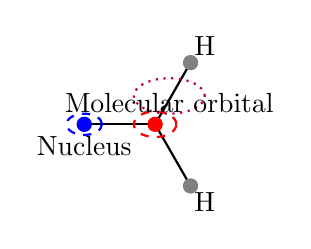
\begin{tikzpicture}[scale=0.9]
        % Draw molecule
        \draw[thick] (0,0) -- (1,0);
        \draw[thick] (1,0) -- (1.5,0.87);
        \draw[thick] (1,0) -- (1.5,-0.87);
        \filldraw[blue] (0,0) circle (0.1);
        \filldraw[red] (1,0) circle (0.1);
        \filldraw[gray] (1.5,0.87) circle (0.1);
        \filldraw[gray] (1.5,-0.87) circle (0.1);
        % Draw orbitals
        \draw[thick, dashed, blue] (0,0) ellipse (0.25 and 0.15);
        \draw[thick, dashed, red] (1,0) ellipse (0.3 and 0.18);
        % Electron cloud
        \draw[thick, dotted, purple] (1.2,0.4) ellipse (0.5 and 0.25);
        % Labels
        \node at (0,-0.3) {Nucleus};
        \node at (1.7,1.1) {H};
        \node at (1.7,-1.1) {H};
        \node at (1.2,0.3) {Molecular orbital};
    \end{tikzpicture}
\end{frame}

\begin{frame}{\huge CC2}\large
	Second-order approximate coupled-cluster singles and doubles (CC2) method is obtained from a perturbative analysis of the CCSD model
	\vspace{5pt}
	\begin{itemize}
		\item Lowers computational scaling from CCSD 
		\item Allows treatment of “big” molecules: $>$ 25 heavy atoms
	\end{itemize}
	\centering
	\vspace{30pt}
	\begin{table}
		\centering
		\begin{tabular}{lcc}\toprule
		\textbf{Method} & \textbf{Scaling} & \textbf{Memory}\\\midrule
		CCSD & $O(N^6)$ & $O(N^{4})^*$\\
		CC2 & $O(N^5)$ & $O(N^{4})^*$\\\bottomrule
		\multicolumn{3}{l}{\small $^*\,O(N^3)$ with RI approximation.}
		\end{tabular}
	\end{table}
\end{frame}

\begin{frame}{\huge Quantum chemical methods}\large
	The time independent Schrödinger equation is approximatelly solved to describe the electronic structure of molecules:
	\begin{equation*}
		\hat{H} \Psi = E \Psi
	\end{equation*}
	We construct the wavefunction $\Psi$ as a combination of molecular orbitals (MOs):
	\begin{equation*}
		\Psi = \sum_{i} c_i \phi_i
	\end{equation*}
\end{frame}
\fi

\end{document}
